\section{Selection and Optimization}

The events analyzed in this dissertation are selected based on requirements for the numbers and types of different reconstructed objects and the relationships between those objects within each event. The selection criteria are applied in three stages. The most basic criteria are applied first in the preselection. This stage is used to validate the Monte Carlo background simulations by examining various relevant kinematic distributions. Second, additional criteria are applied in the main selection, which more closely addresses the expected properties of signal events. Kinematic distributions in the main selection are used to optimize the cuts for the final selection, in order to reduce the contributions from background while enhancing the signal. These optimizations maximize the expected limit from the MC background simulations. Separate final selections are defined for the leptoquark search and the top squark search.

\subsection{Preselection}

At the preselection stage, a single primary well-identified light lepton $\ell$ is required. In the \etau channel, this is an electron satisfying the medium working point and kinematic criteria described in Sec. \ref{sec:ele-reco}. In the \mutau channel, this is a muon satisfying the tight working point and kinematic criteria described in Sec. \ref{sec:muon-reco}. In addition to the light lepton, the event must contain a hadronic tau identified by the HPS algorithm and associated discriminators as defined in Sec. \ref{sec:hpstau}. The two objects, light lepton and hadronic tau, must have opposite charges, originate from the same vertex, and be separated by $\Delta R > 0.5$. Two jets are also required, satisfying the loose working point and kinematic criteria described in Sec. \ref{sec:jet-reco}. The jets must be separated from the light lepton and the hadronic tau by $\Delta R > 0.5$.

Several cases of additional light leptons are vetoed. To suppress background from the \Z + jets process, events are rejected if they contain additional light leptons satisfying the loose working point and having the same flavor and opposite charge with respect to the primary lepton. This separates the contributions from the $\Z \rightarrow \ell\ell$+jets process into control regions which will be used for background estimation. To avoid overlap between the two channels, events are rejected if they contain additional light leptons satisfying the primary working point and kinematic criteria for leptons (medium for electrons and tight for muons) and having the opposite flavor and opposite charge with respect to the primary lepton. This also defines an \emu control region which will be used for background estimation.

Figures \ref{fig:preseletau} and \ref{fig:preselmutau} compare the observed data to the MC background simulation after the preselection in the \etau and \mutau channels, respectively. All histograms in this dissertation show the overflow, if any, in the last bin. The event yields for the observed data and the expected SM backgrounds after the preselection are summarized in Table \ref{tab:eventyieldpresel}. The discrepancy between the observed data and simulated background yields in the \etau channel is due to the presence of QCD multijet events in the observed data. This discrepancy is primarily observed at low \pt and high $\eta$, as expected from QCD. This process is not modeled in the MC simulation because of the difficulty in simulating enough events to be comparable to the amount of data collected by the CMS experiment in 2012. Instead, the yield from QCD is estimated using a same-sign/opposite-sign method which is described in detail in Sec. \ref{sec:qcdbkg}.

\begin{figure}[hbtp]
  \begin{center}
    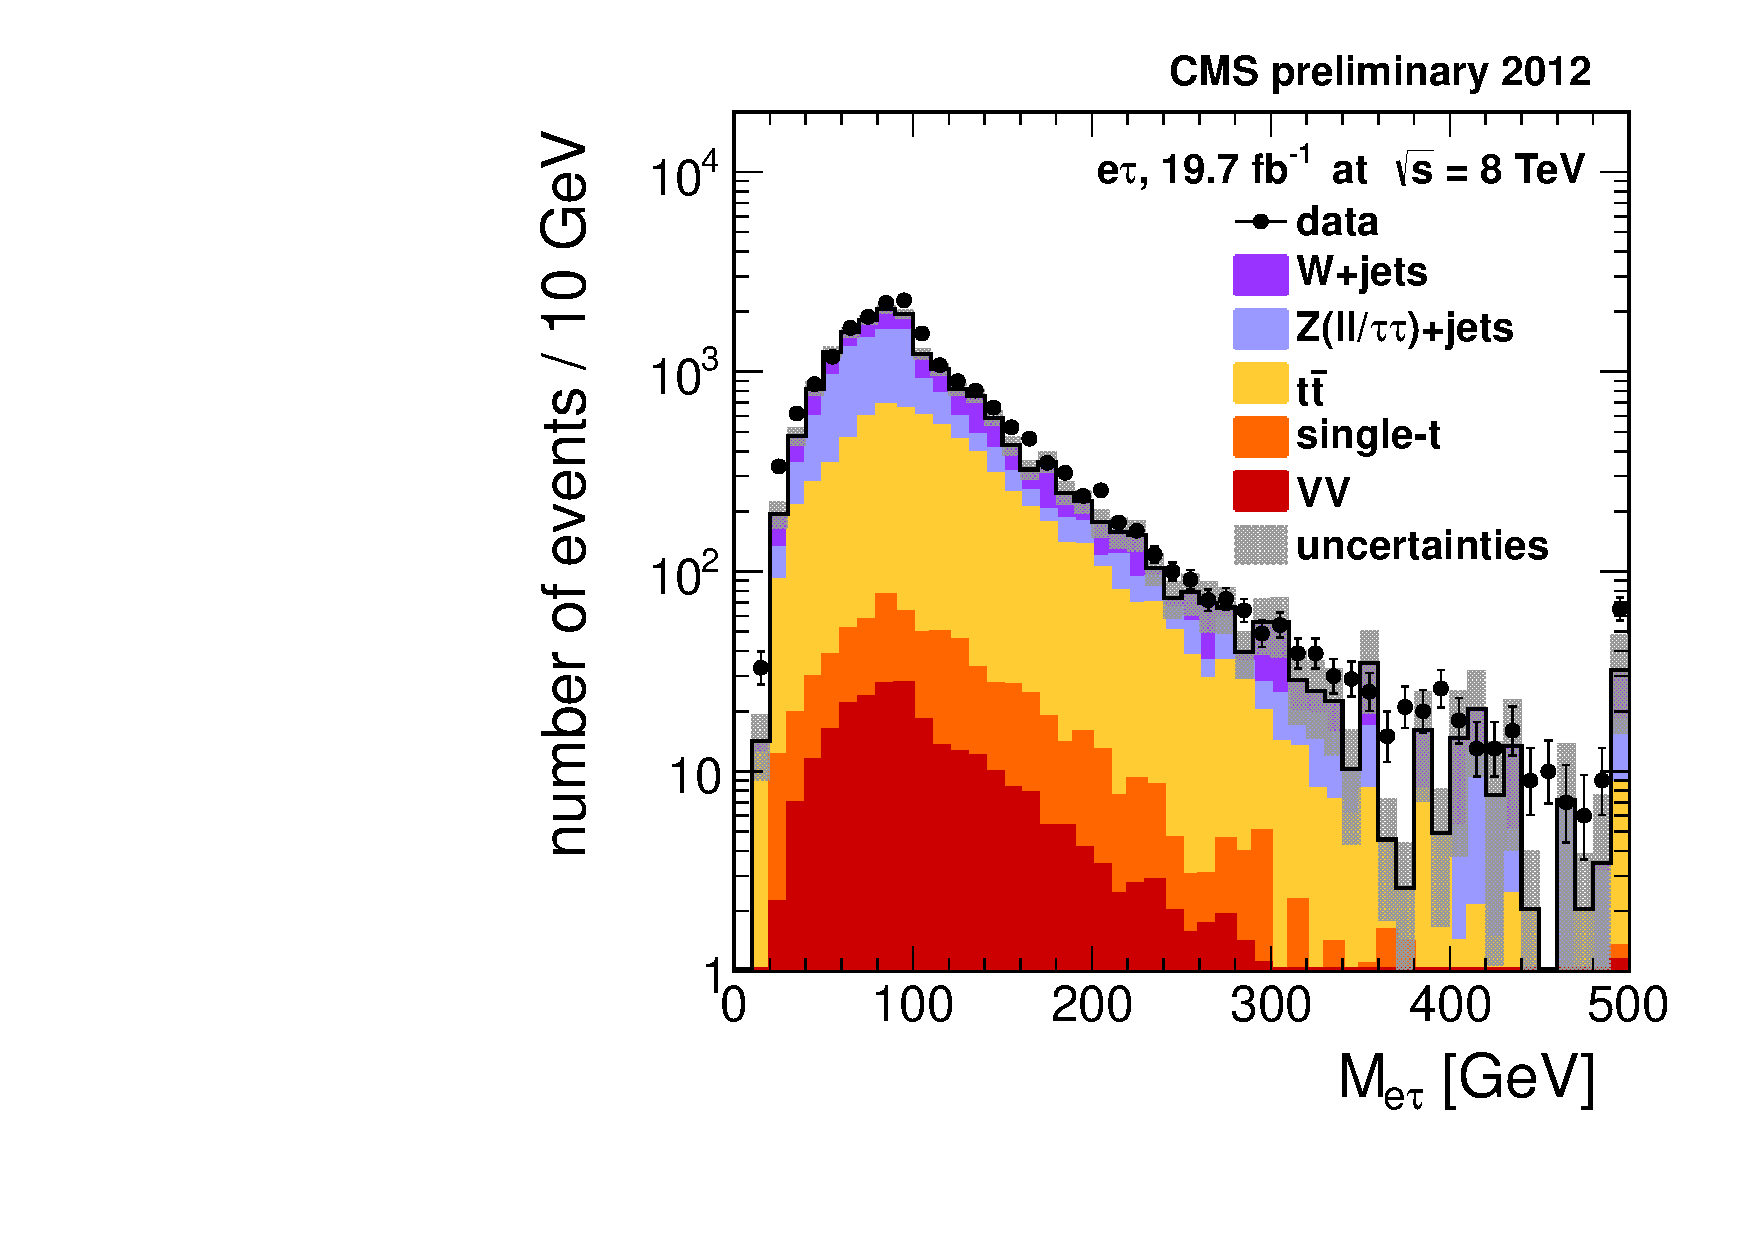
\includegraphics[width=0.465\textwidth]{figures/etau/etauMassMultJet.pdf}
    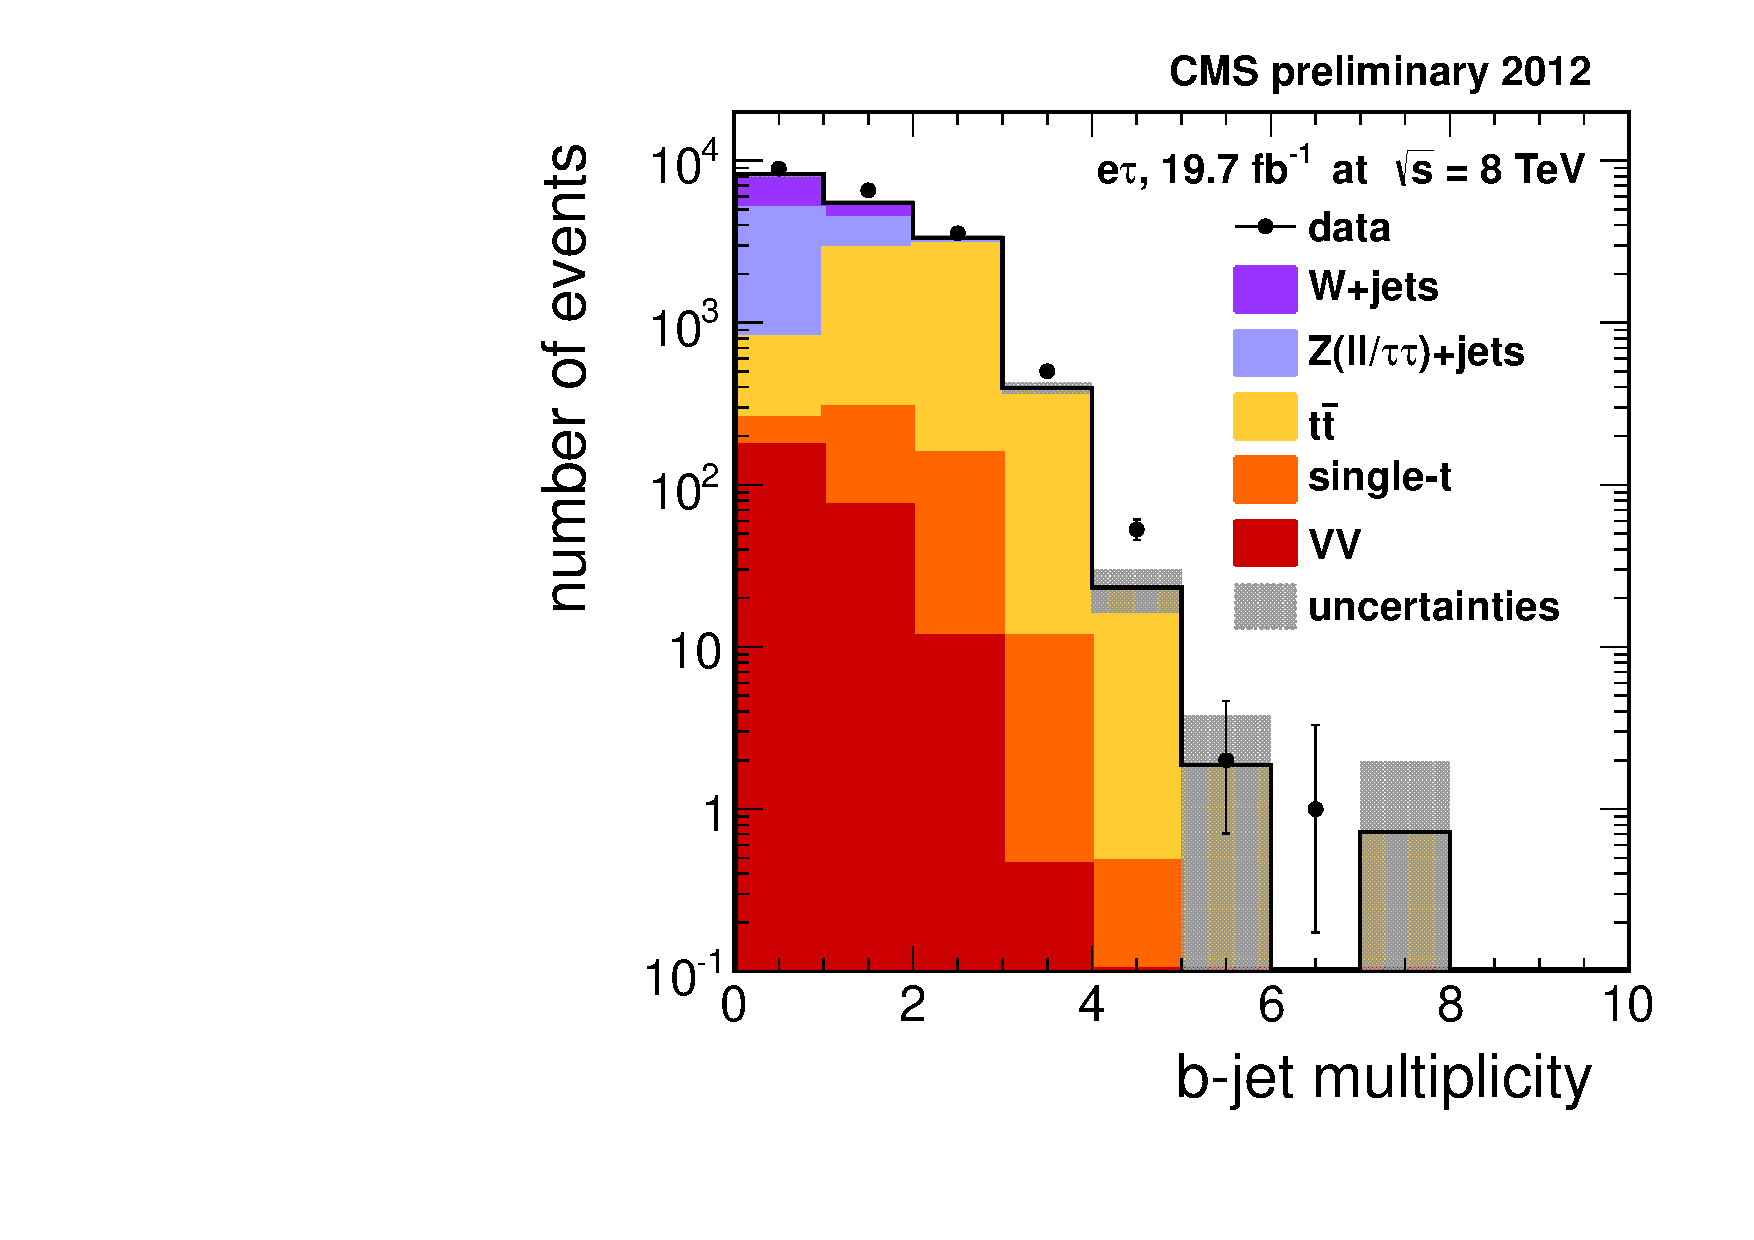
\includegraphics[width=0.465\textwidth]{figures/etau/nBJetMultJet.pdf} \\
    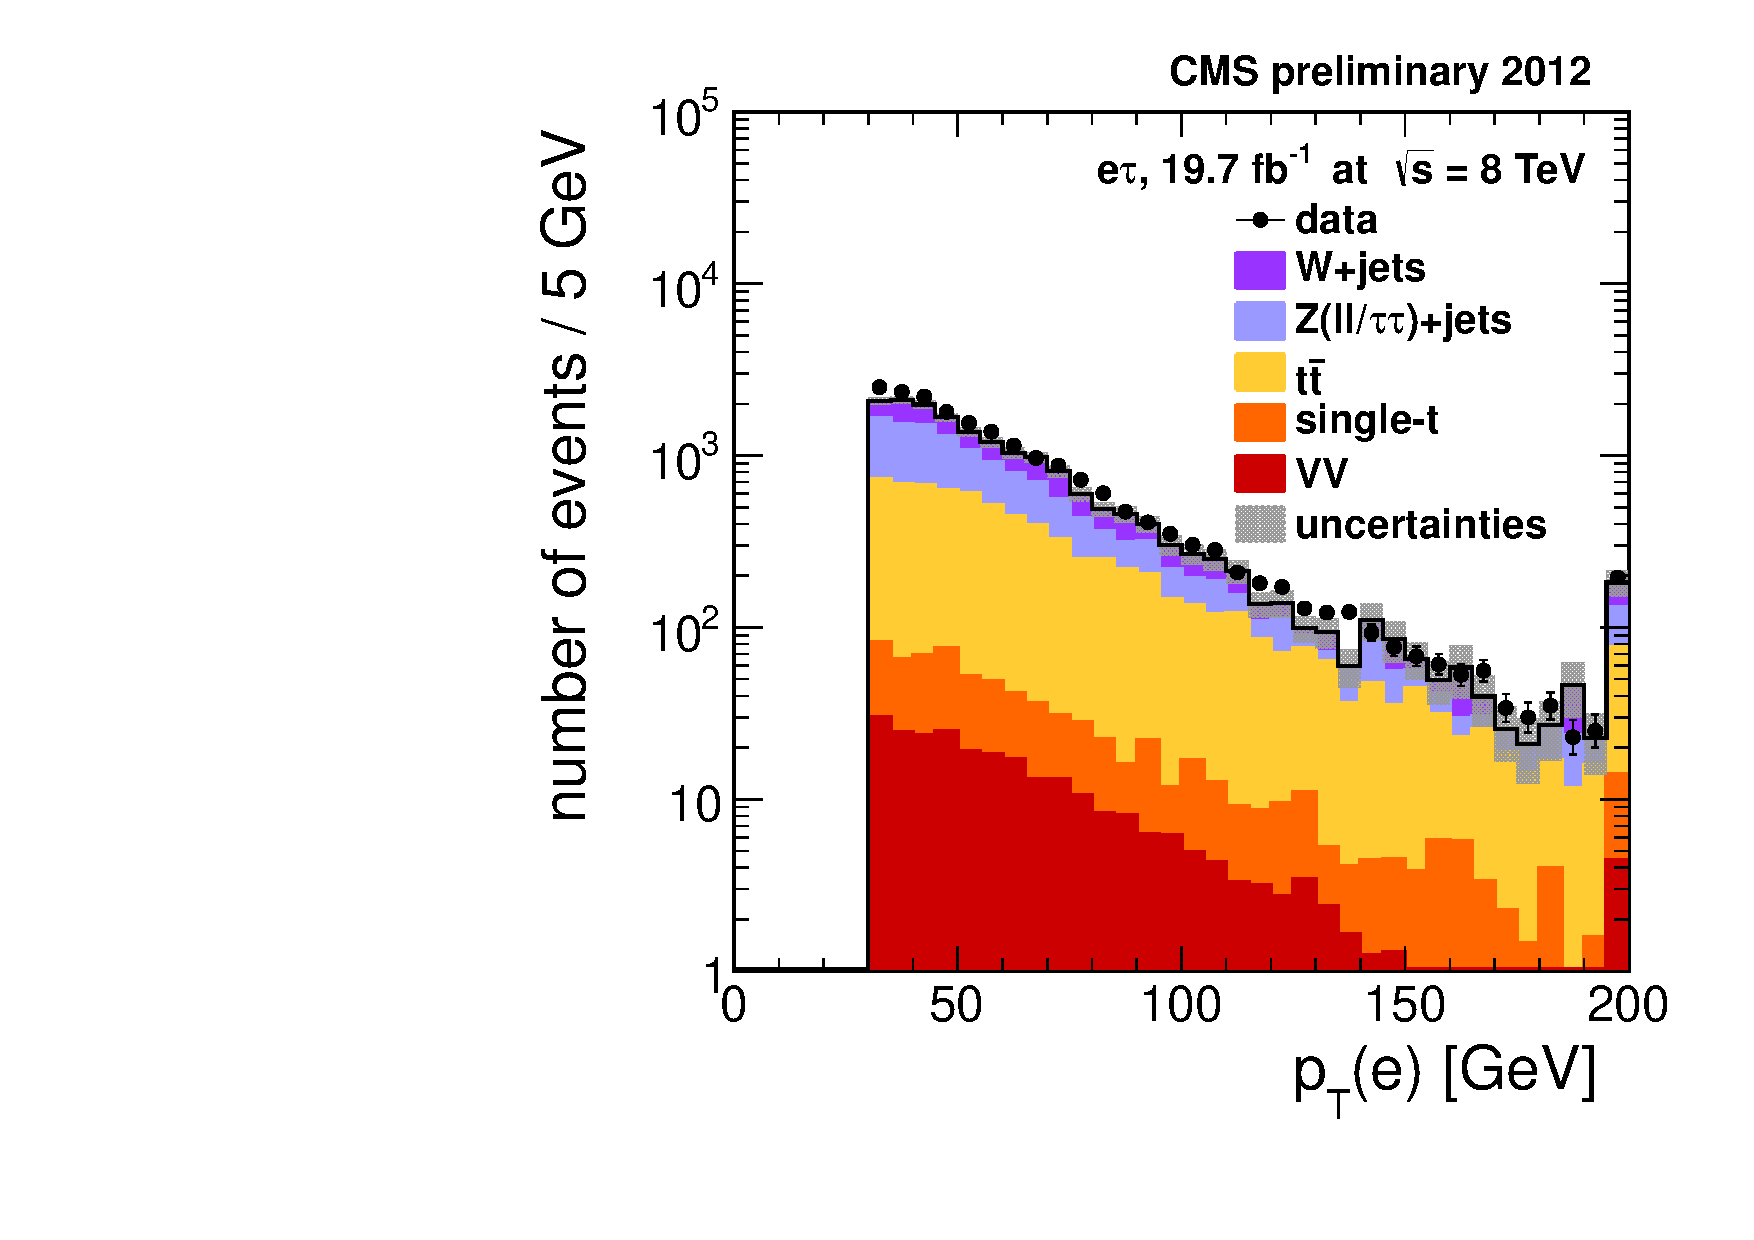
\includegraphics[width=0.465\textwidth]{figures/etau/elPtMultJet.pdf}
    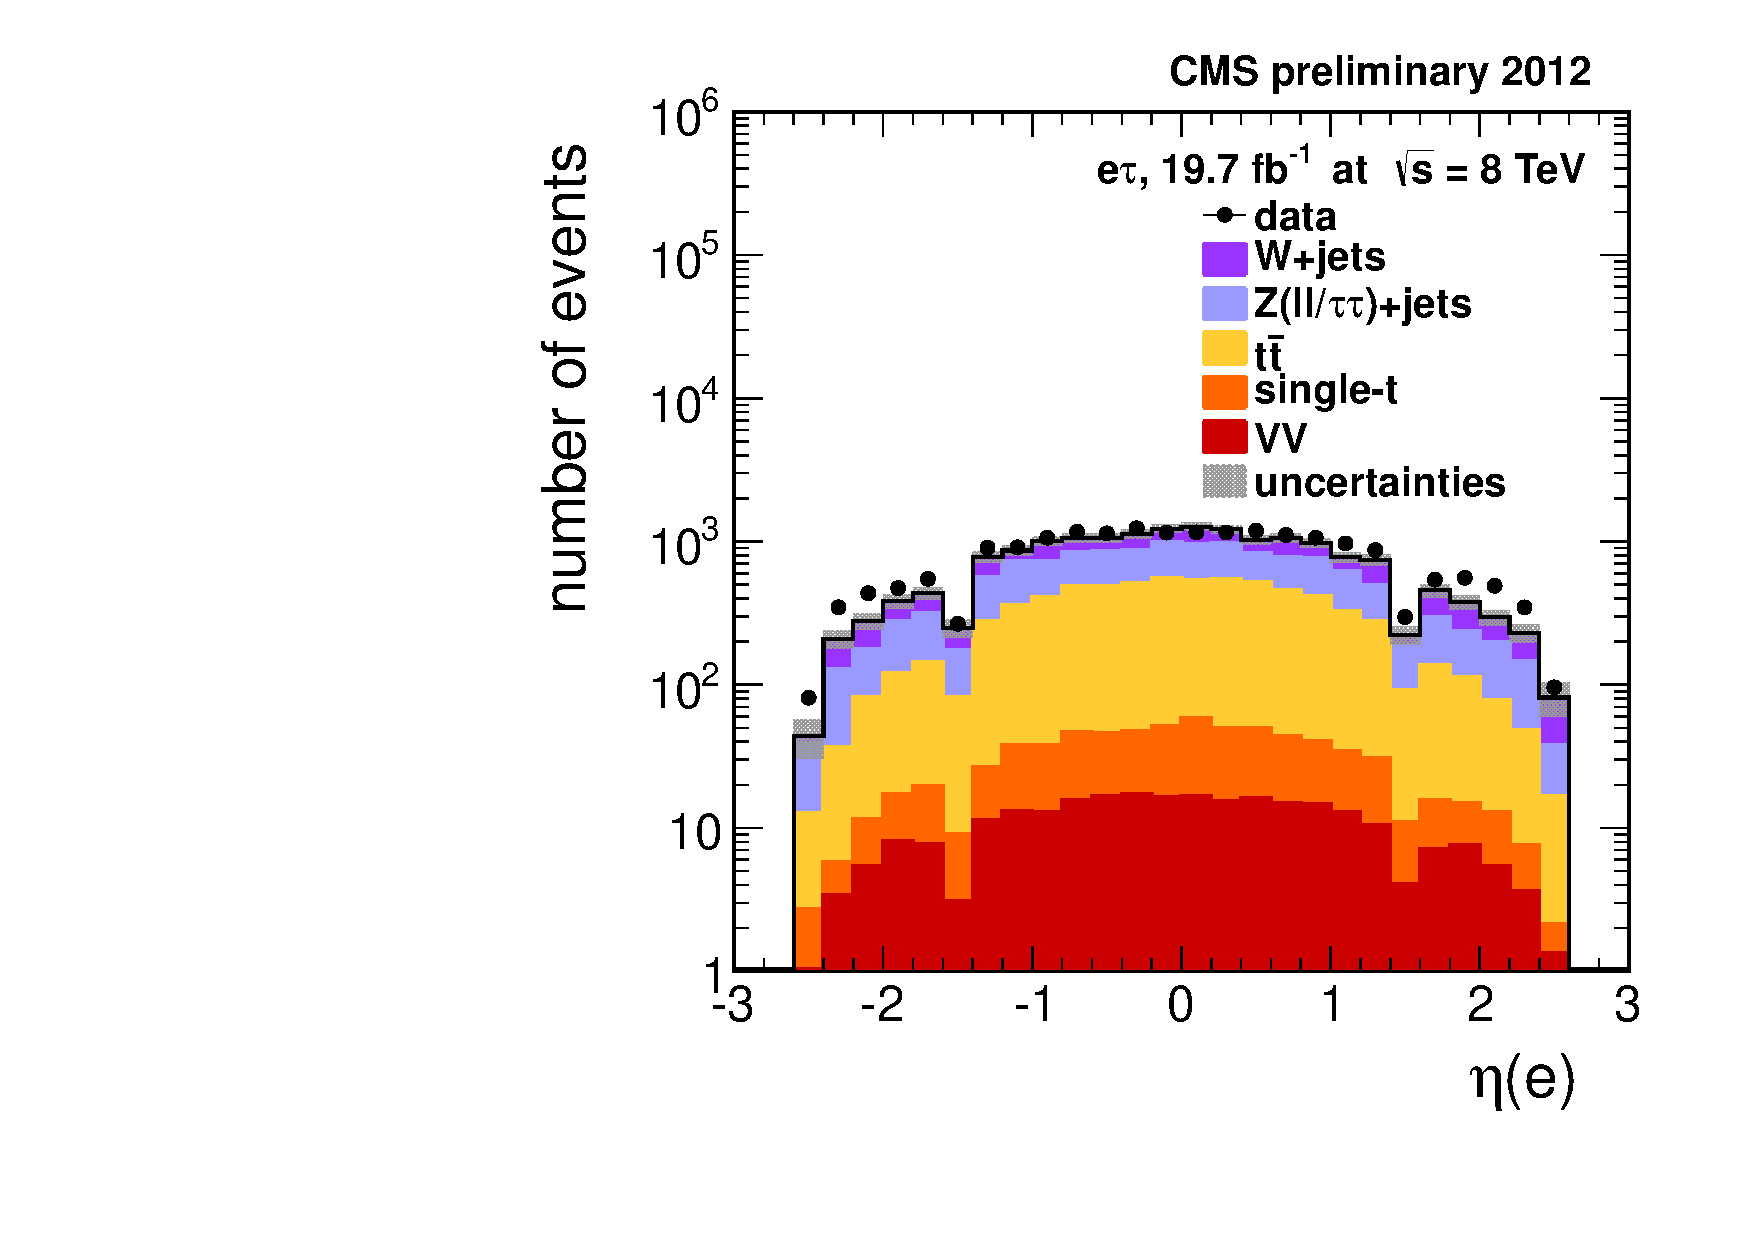
\includegraphics[width=0.465\textwidth]{figures/etau/elEtaMultJet.pdf} \\
    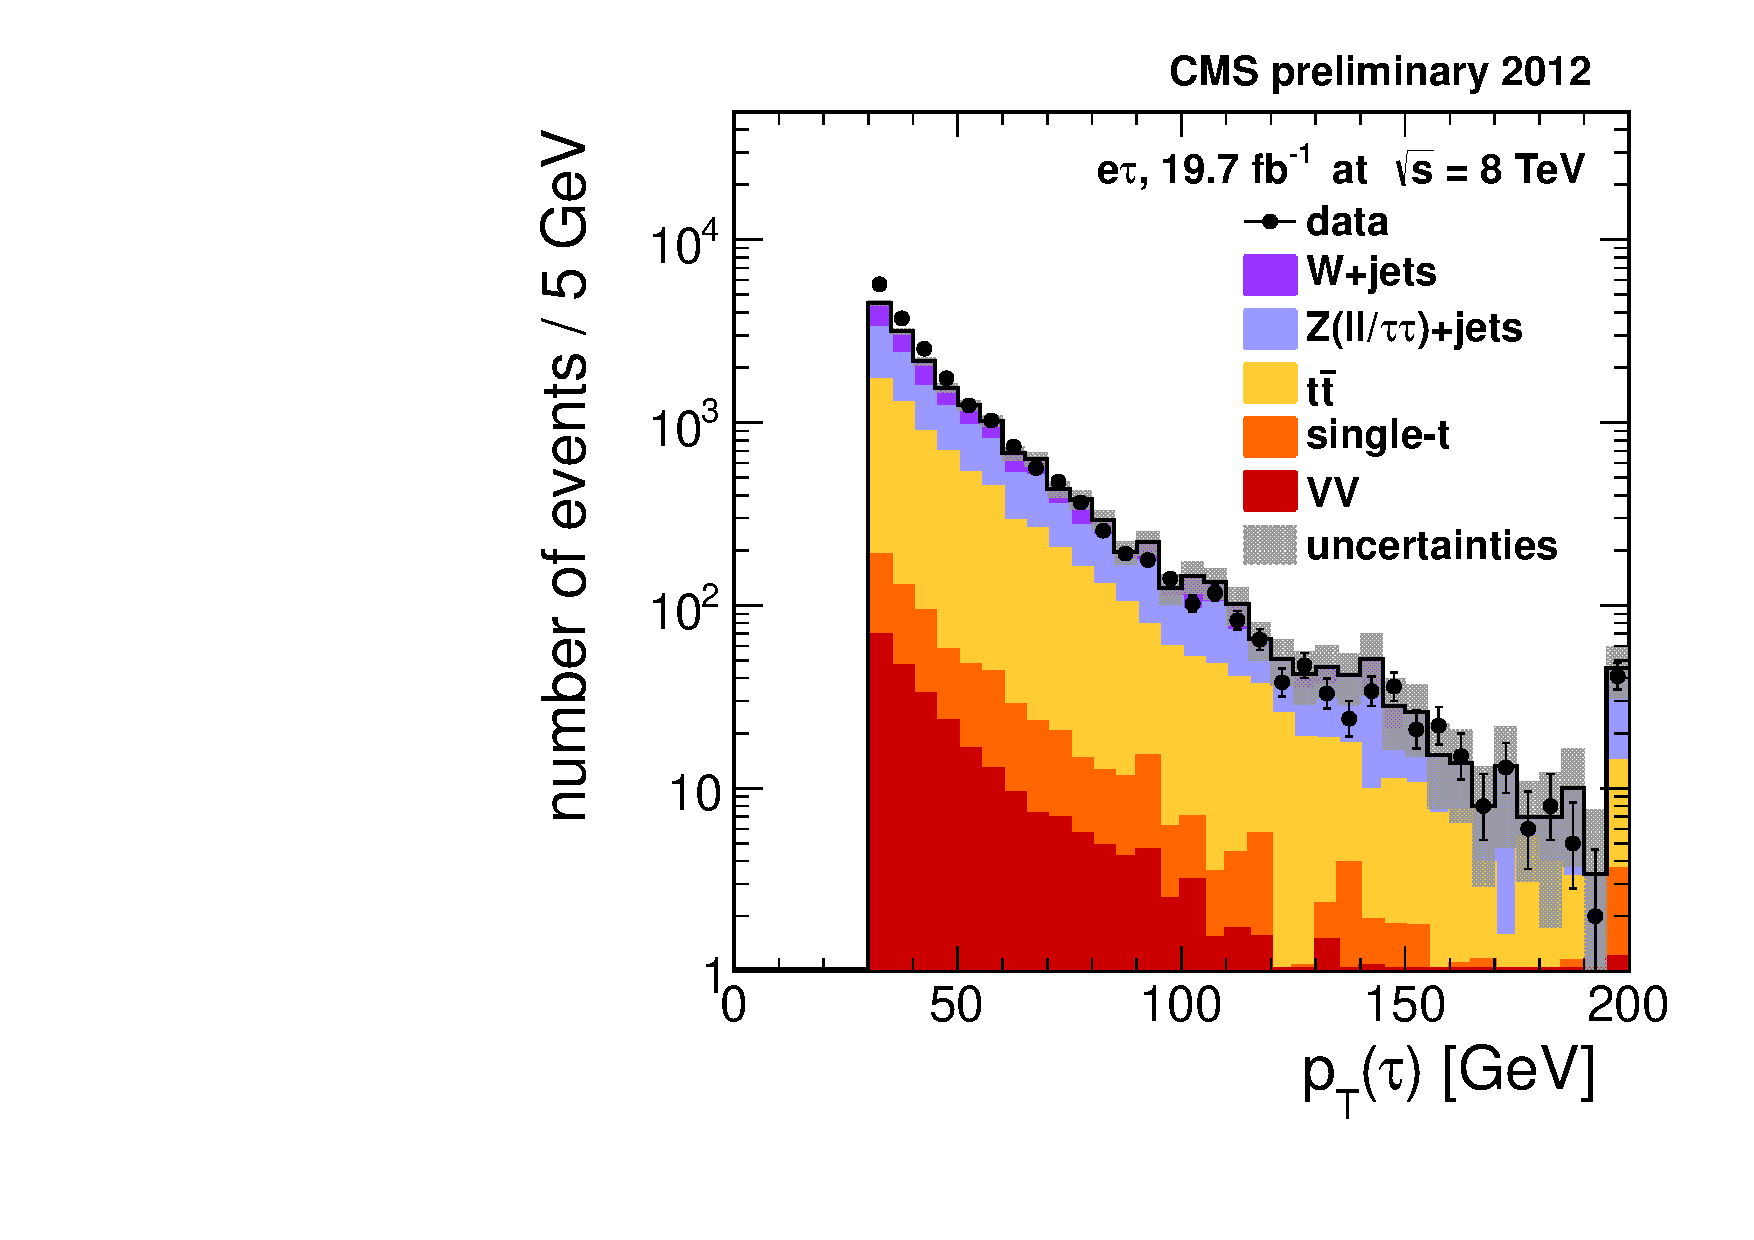
\includegraphics[width=0.465\textwidth]{figures/etau/tauPtMultJet.pdf}
    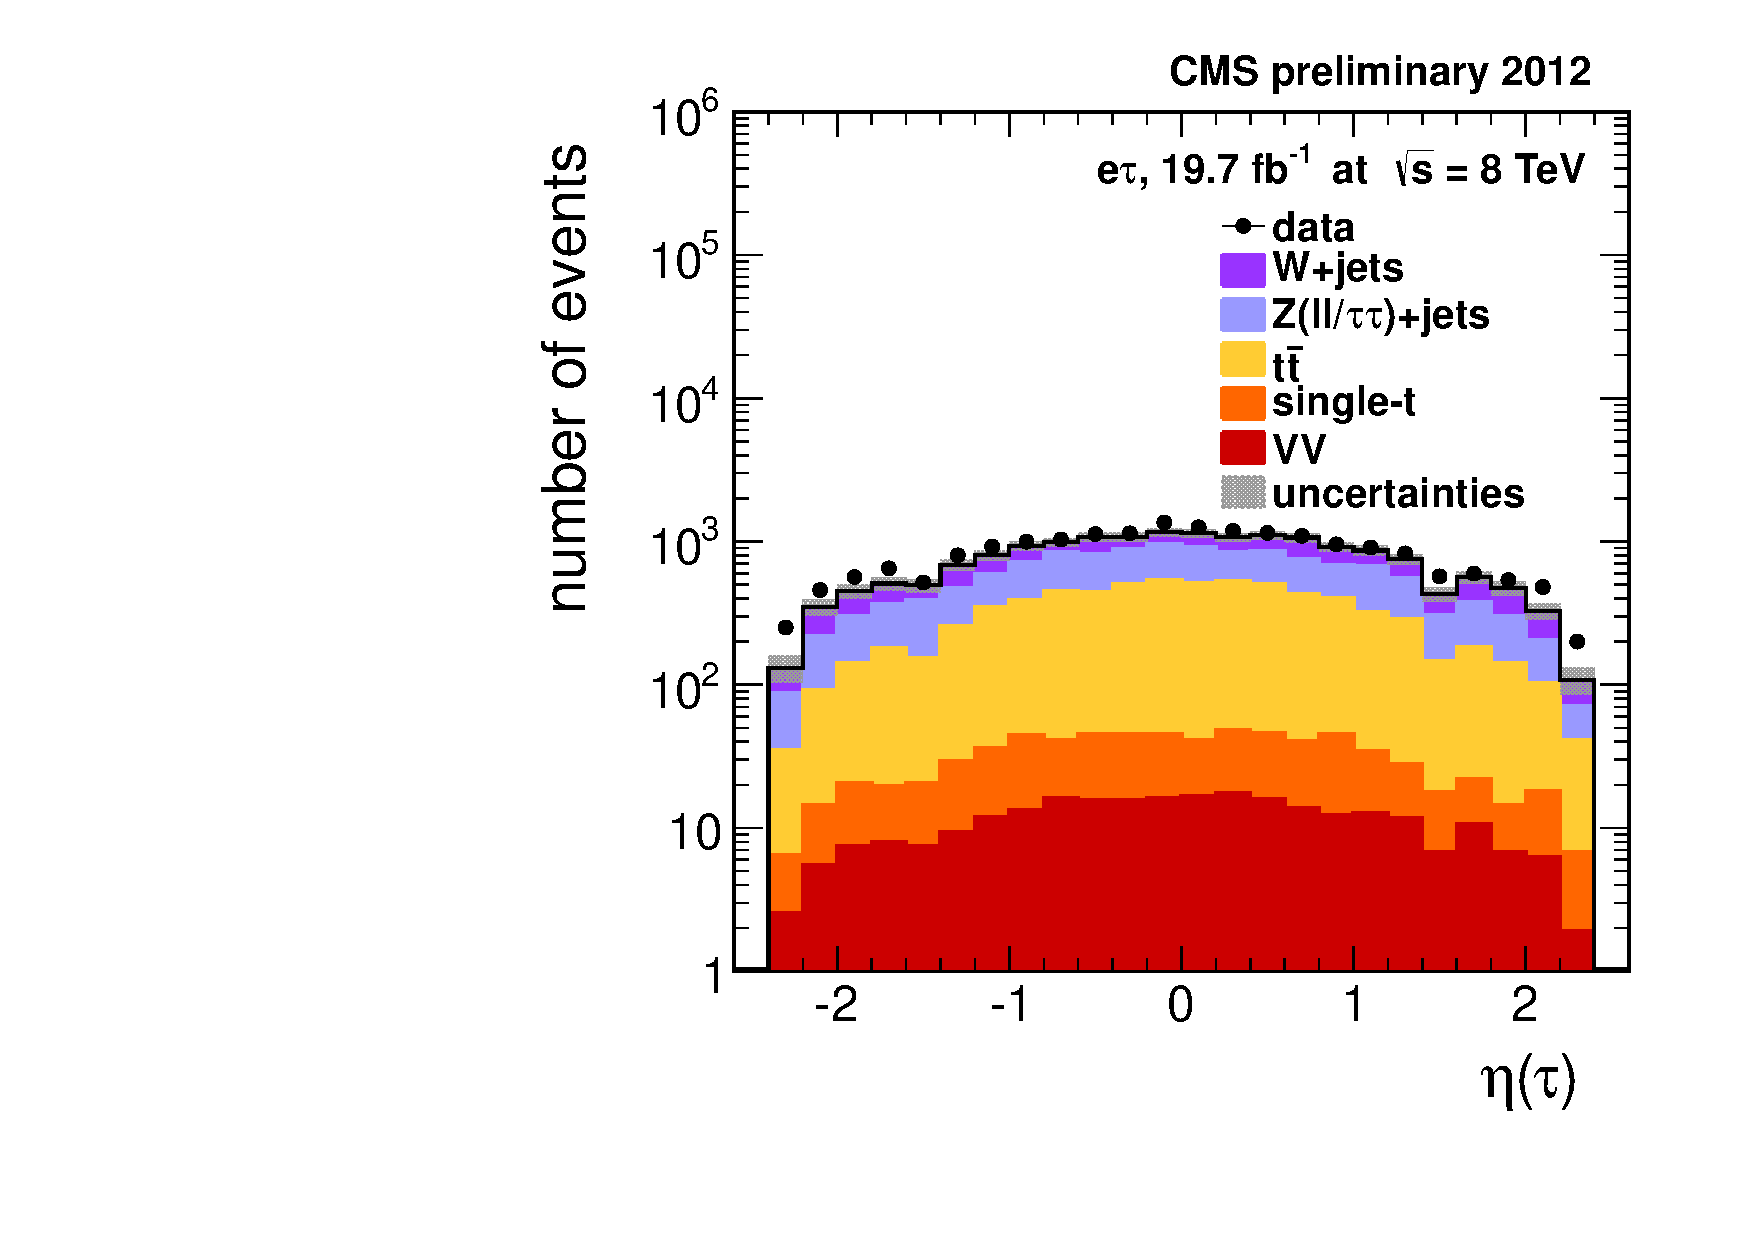
\includegraphics[width=0.465\textwidth]{figures/etau/tauEtaMultJet.pdf}
    \caption{Plots of various kinematic quantities comparing observed data and simulated backgrounds in the \etau channel after the preselection: the visible mass of the electron and hadronic tau (top left), the number of b-tagged jets (top right), the \pt (left) and $\eta$ (right) of the electron (middle) and hadronic tau (bottom). The uncertainty band reflects the statistical uncertainty in the simulated backgrounds.}
    \label{fig:preseletau}
  \end{center}
\end{figure}

\begin{figure}[hbtp]
  \begin{center}
    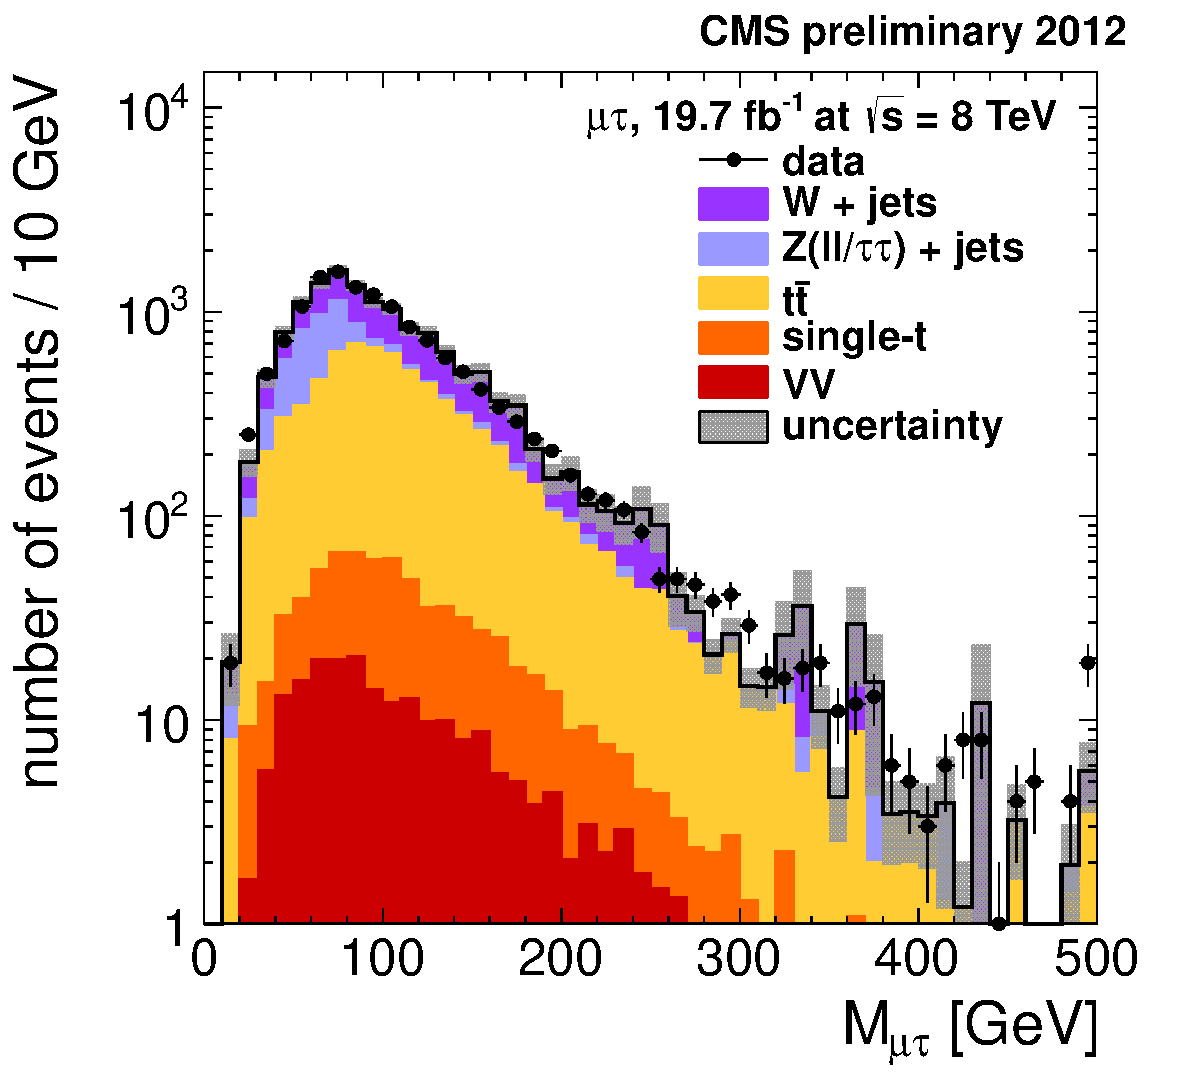
\includegraphics[width=0.465\textwidth]{figures/mutau/preselection/mass.pdf}
    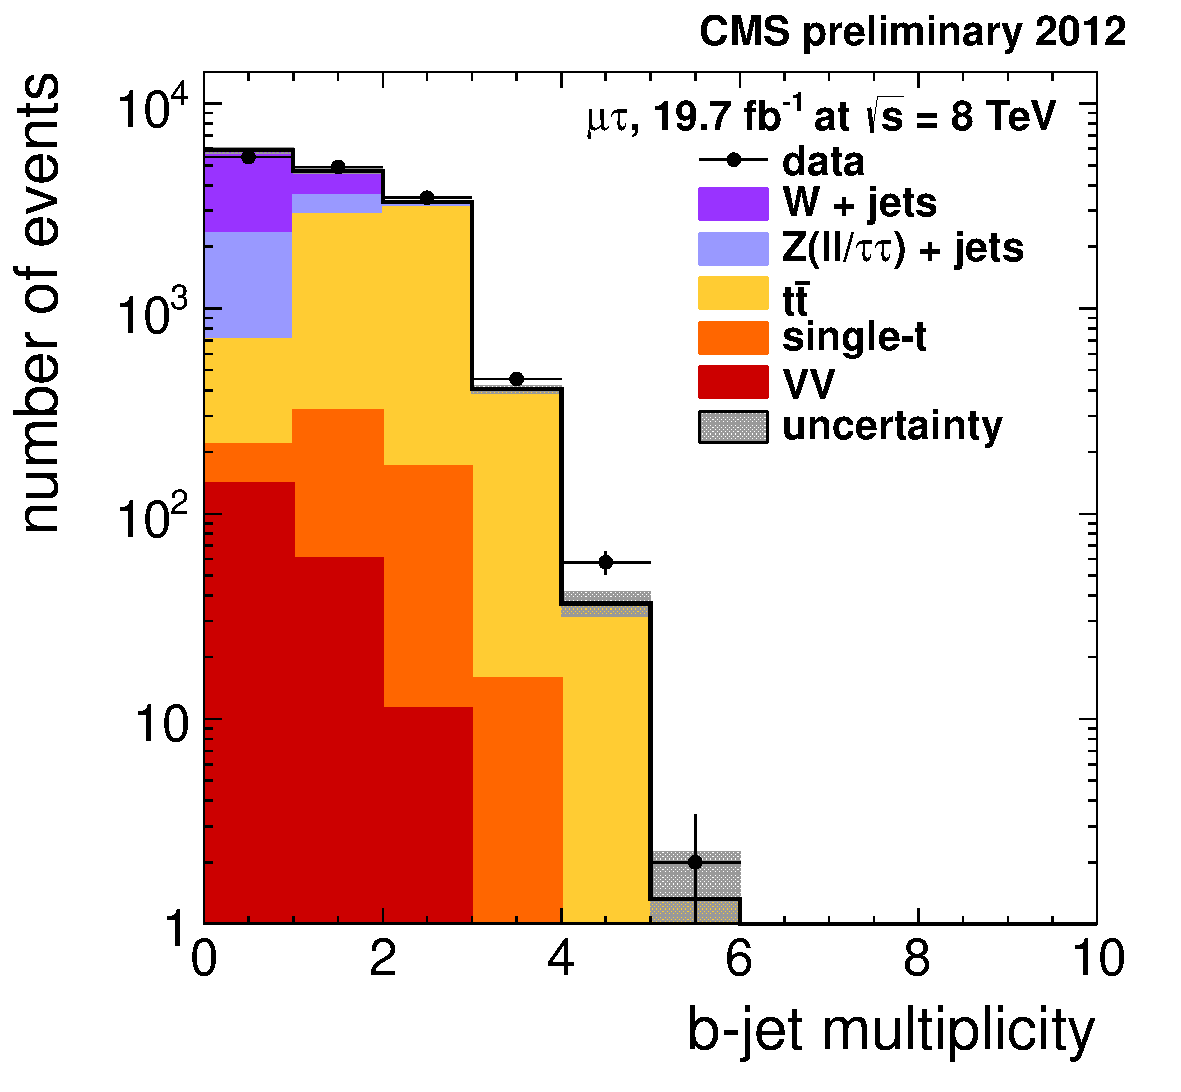
\includegraphics[width=0.465\textwidth]{figures/mutau/preselection/nbjet.pdf} \\
    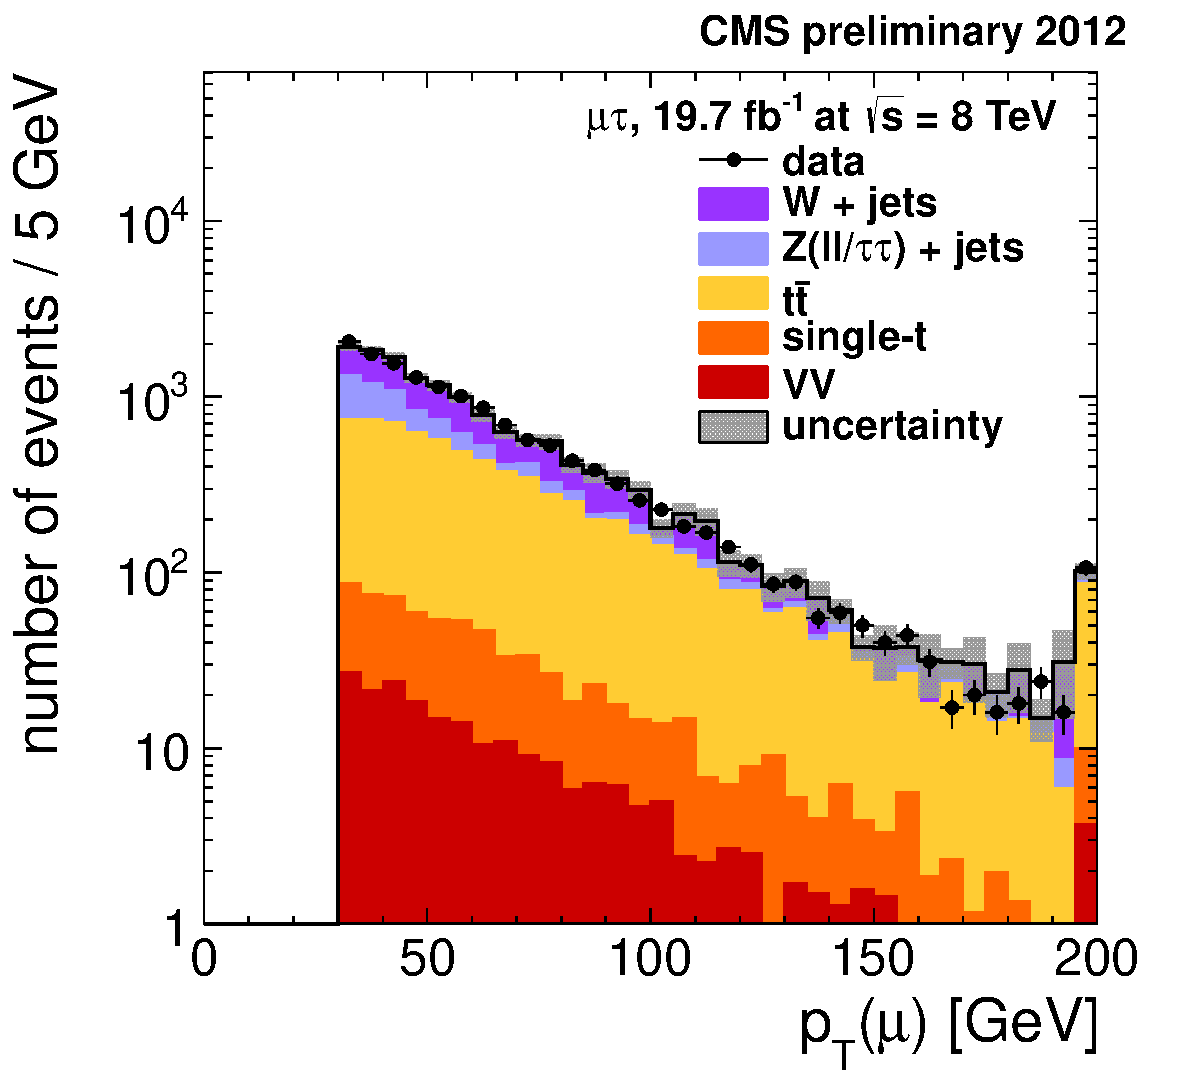
\includegraphics[width=0.465\textwidth]{figures/mutau/preselection/ptmu.pdf}
    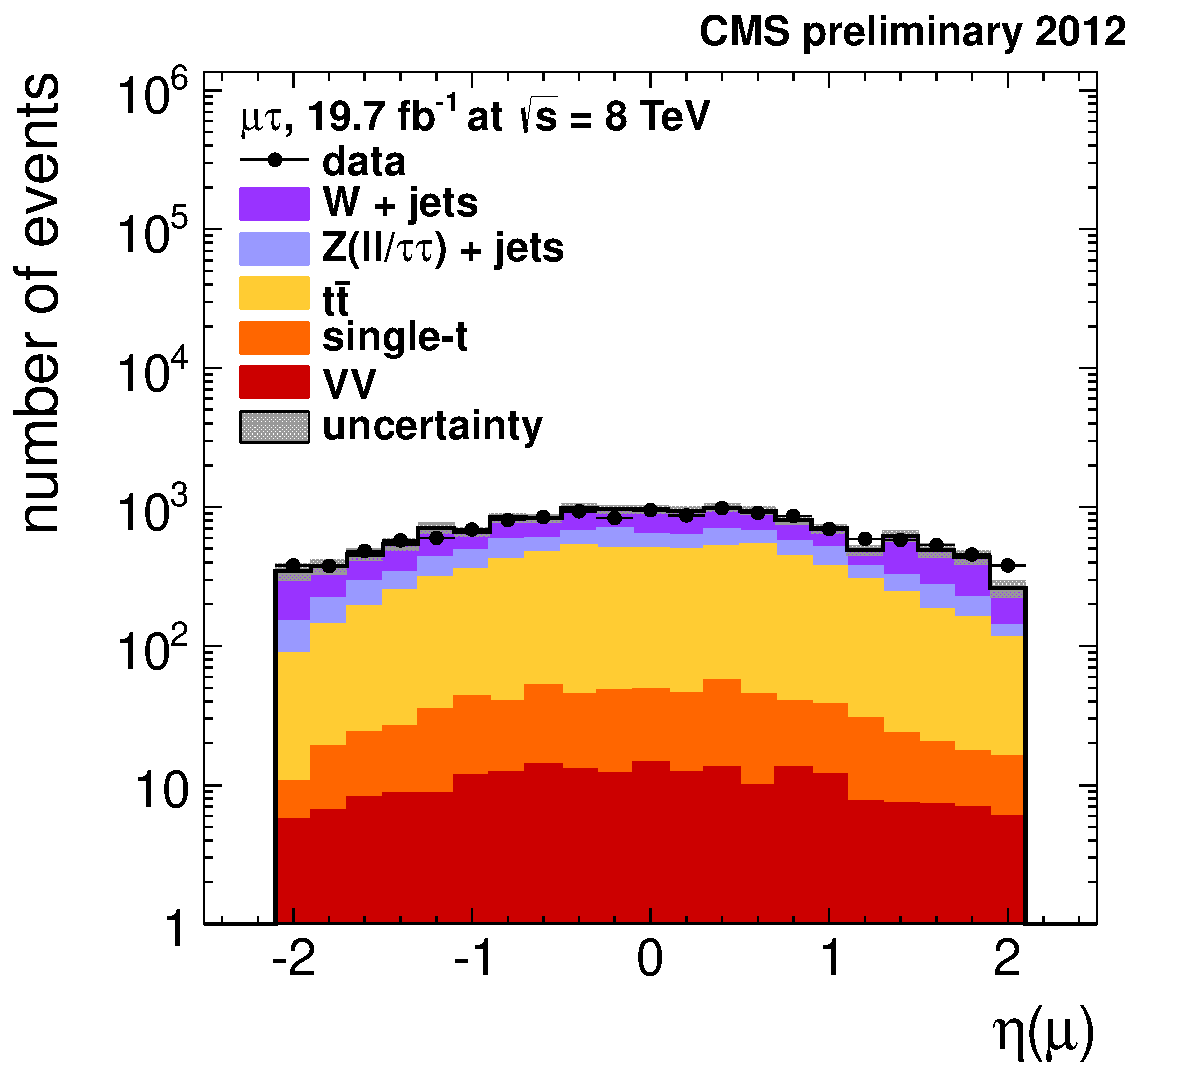
\includegraphics[width=0.465\textwidth]{figures/mutau/preselection/etamu.pdf} \\
    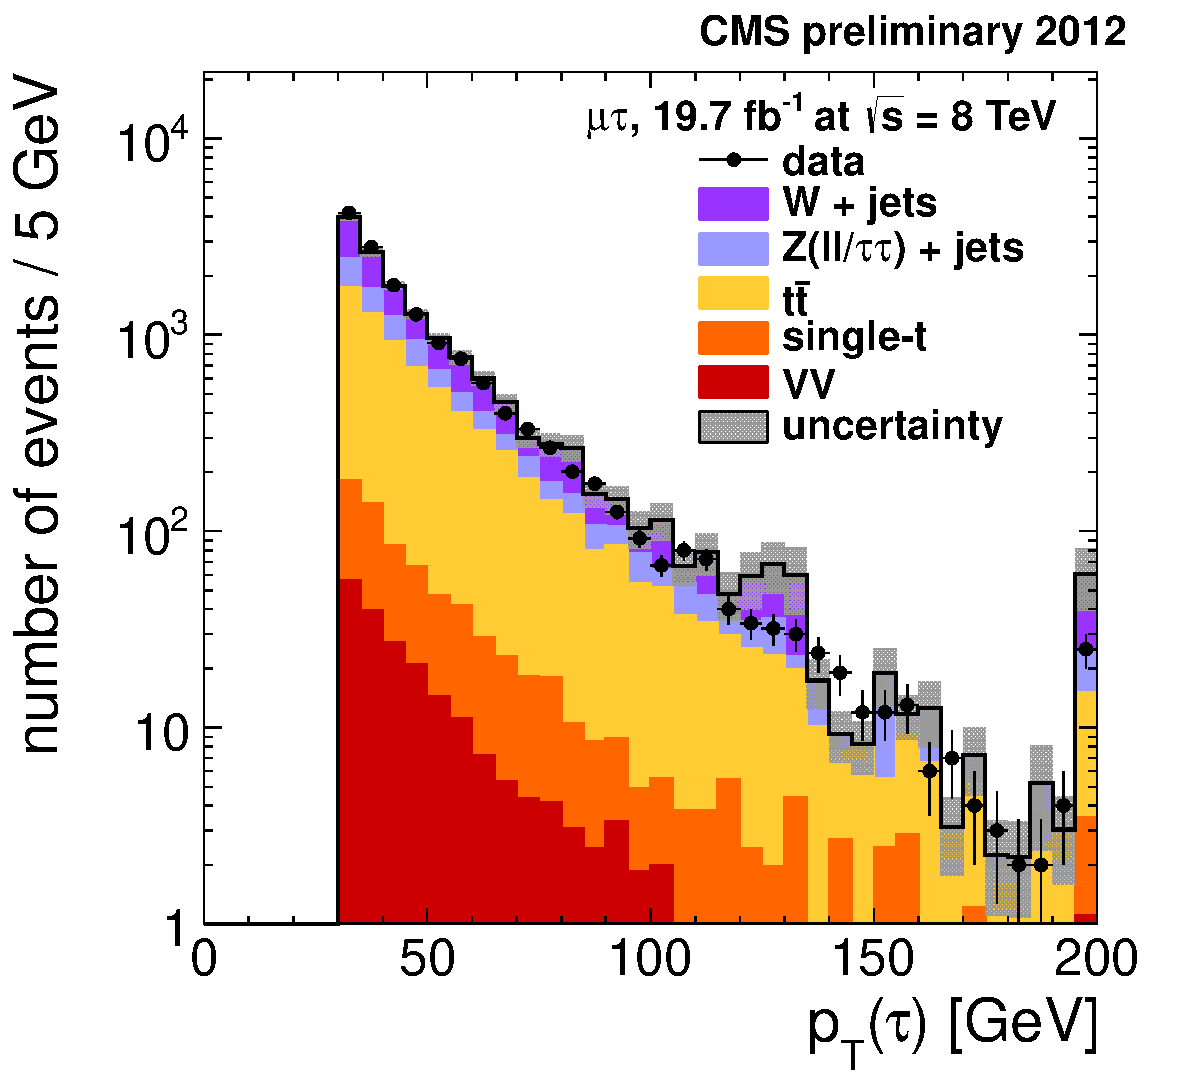
\includegraphics[width=0.465\textwidth]{figures/mutau/preselection/pttau.pdf}
    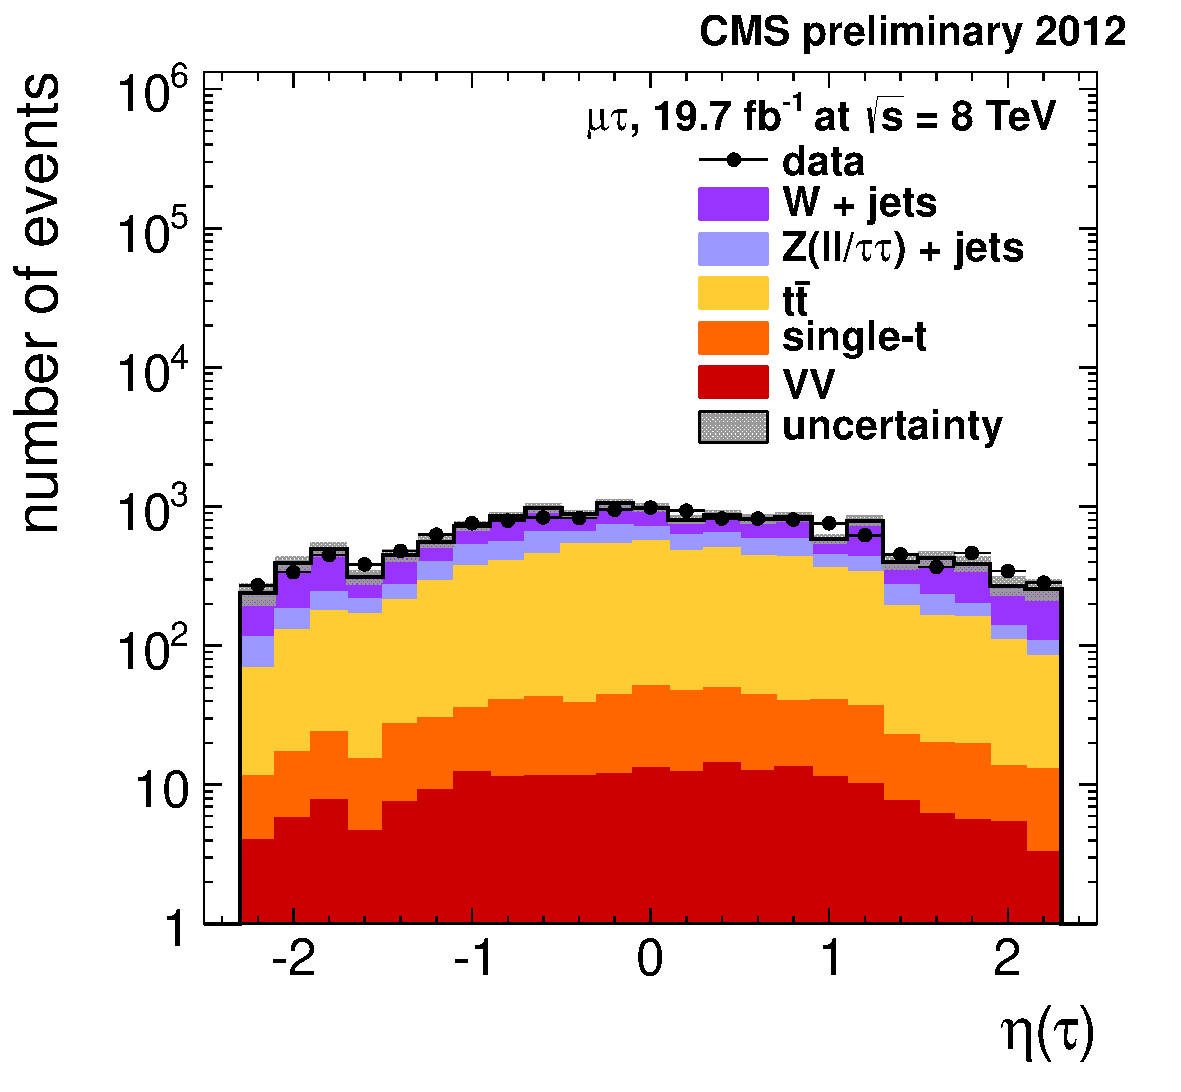
\includegraphics[width=0.465\textwidth]{figures/mutau/preselection/etatau.pdf}
    \caption{Plots of various kinematic quantities comparing observed data and simulated backgrounds in the \mutau channel after the preselection: the visible mass of the muon and hadronic tau (top left), the number of b-tagged jets (top right), the \pt (left) and $\eta$ (right) of the muon (middle) and hadronic tau (bottom). The uncertainty band reflects the statistical uncertainty in the simulated backgrounds.}
    \label{fig:preselmutau}
  \end{center}
\end{figure}

\begin{table}[hbt]
  \begin{center}
    \begin{tabular}{|l|r@{$\,\pm\,$}r|r@{$\,\pm\,$}r|}
      \hline
      & \multicolumn{2}{c|}{\etau channel} & \multicolumn{2}{c|}{\mutau channel} \\
      \hline
      \W + jets                       &  4221.6 & 188.1   & 4846.3 & 233.6  \\
      \Z + jets                       &  4766.7 & 85.1    & 2369.1 & 80.7   \\
      \ttbar                          &  6272.2 & 65.5    & 6430.5 & 69.8   \\
      Single \cPqt                    &  462.9 & 14.4     & 512.3 & 16.0    \\
      VV                              &  223.4 & 4.4      & 212.5 & 4.6     \\
      QCD multijets                   &  (2452.6 & 512.1)\neghphantom{)} & \multicolumn{2}{c|}{---} \\ 
      \hline                                                  
      Total Bkg. (no QCD)             & 15946.8 & 232.9   & 14370.8 & 257.3 \\
      \hline                                                  
      \hline                                                  
      Data                            & \multicolumn{1}{r@{\hphantom{$\,\pm\,$}}}{18177\hphantom{.0}} & & \multicolumn{1}{r@{\hphantom{$\,\pm\,$}}}{14351\hphantom{.0}} & \\
      \hline
    \end{tabular}
    \caption{The simulated background and observed event yields after the preselection in the \etau and \mutau channels. The statistical uncertainties are given for each simulated background. The contribution from the QCD multijets process is not taken into account in the total background yield. }
    \label{tab:eventyieldpresel}
  \end{center}
\end{table}

%\clearpage

\subsection{Main Selection}

A preselected event satisfies the main selection if at least one of the selected jets in the event is b-tagged. Though the expected final state from the signal includes two b-jets, it was found that requiring b-tagging for only one jet improved the signal yield in comparison to the SM backgrounds. This is expected due to the reduced efficiency of applying the CSV algorithm for b-tagging multiple times per event. The second jet in the event may or may not be b-tagged. Plots comparing observed data to the simulated backgrounds after the main selection are shown in Figs. \ref{fig:mainseletau} and \ref{fig:mainselmutau}, and event yields are given in Table \ref{tab:eventyieldmainsel}.

At this stage of the selection, several new observables are introduced. The first is the visible mass of the hadronic tau and a jet, \MassTJ. There are two possible pairings of the light lepton and the hadronic tau with the two selected jets. The pairing is chosen to minimize the difference between \MassTJ and \MassLJ. In signal events, these two values are expected to be similar, as both sets of correctly-paired particles will originate from the same mother particles, leptoquarks or top squarks. However, the visible mass variables will not directly measure the true mass of the mother particles; some of the energy will be lost in the form of neutrinos produced in tau lepton decays. According to the simulation of the signal process, this minimization selects the correct pairing in approximately 70\% of events. This observable will be used in the final selection for the leptoquark search.

The second new variable is \ST, which is defined as the scalar sum of \pt for all final-state objects:
\begin{equation}
\label{eq:STLQ}
\ST(\text{LQ}) = \pt(\ell) + \pt(\tauh) + \pt(\text{b-jet}) + \pt(\text{jet}).
\end{equation}
As indicated in Eq. \eqref{eq:STLQ}, this definition of \ST is appropriate for the leptoquark search, which requires four objects in the final state: a light lepton, a hadronic tau, a b-tagged jet, and another jet. Figures \ref{fig:mainseletau} and \ref{fig:mainselmutau} show this version of \ST. An alternate definition appropriate for the top squark search, which has a slightly different final state, is given in Eq. \eqref{eq:STstop}.

\begin{figure}[hbtp]
  \begin{center}
    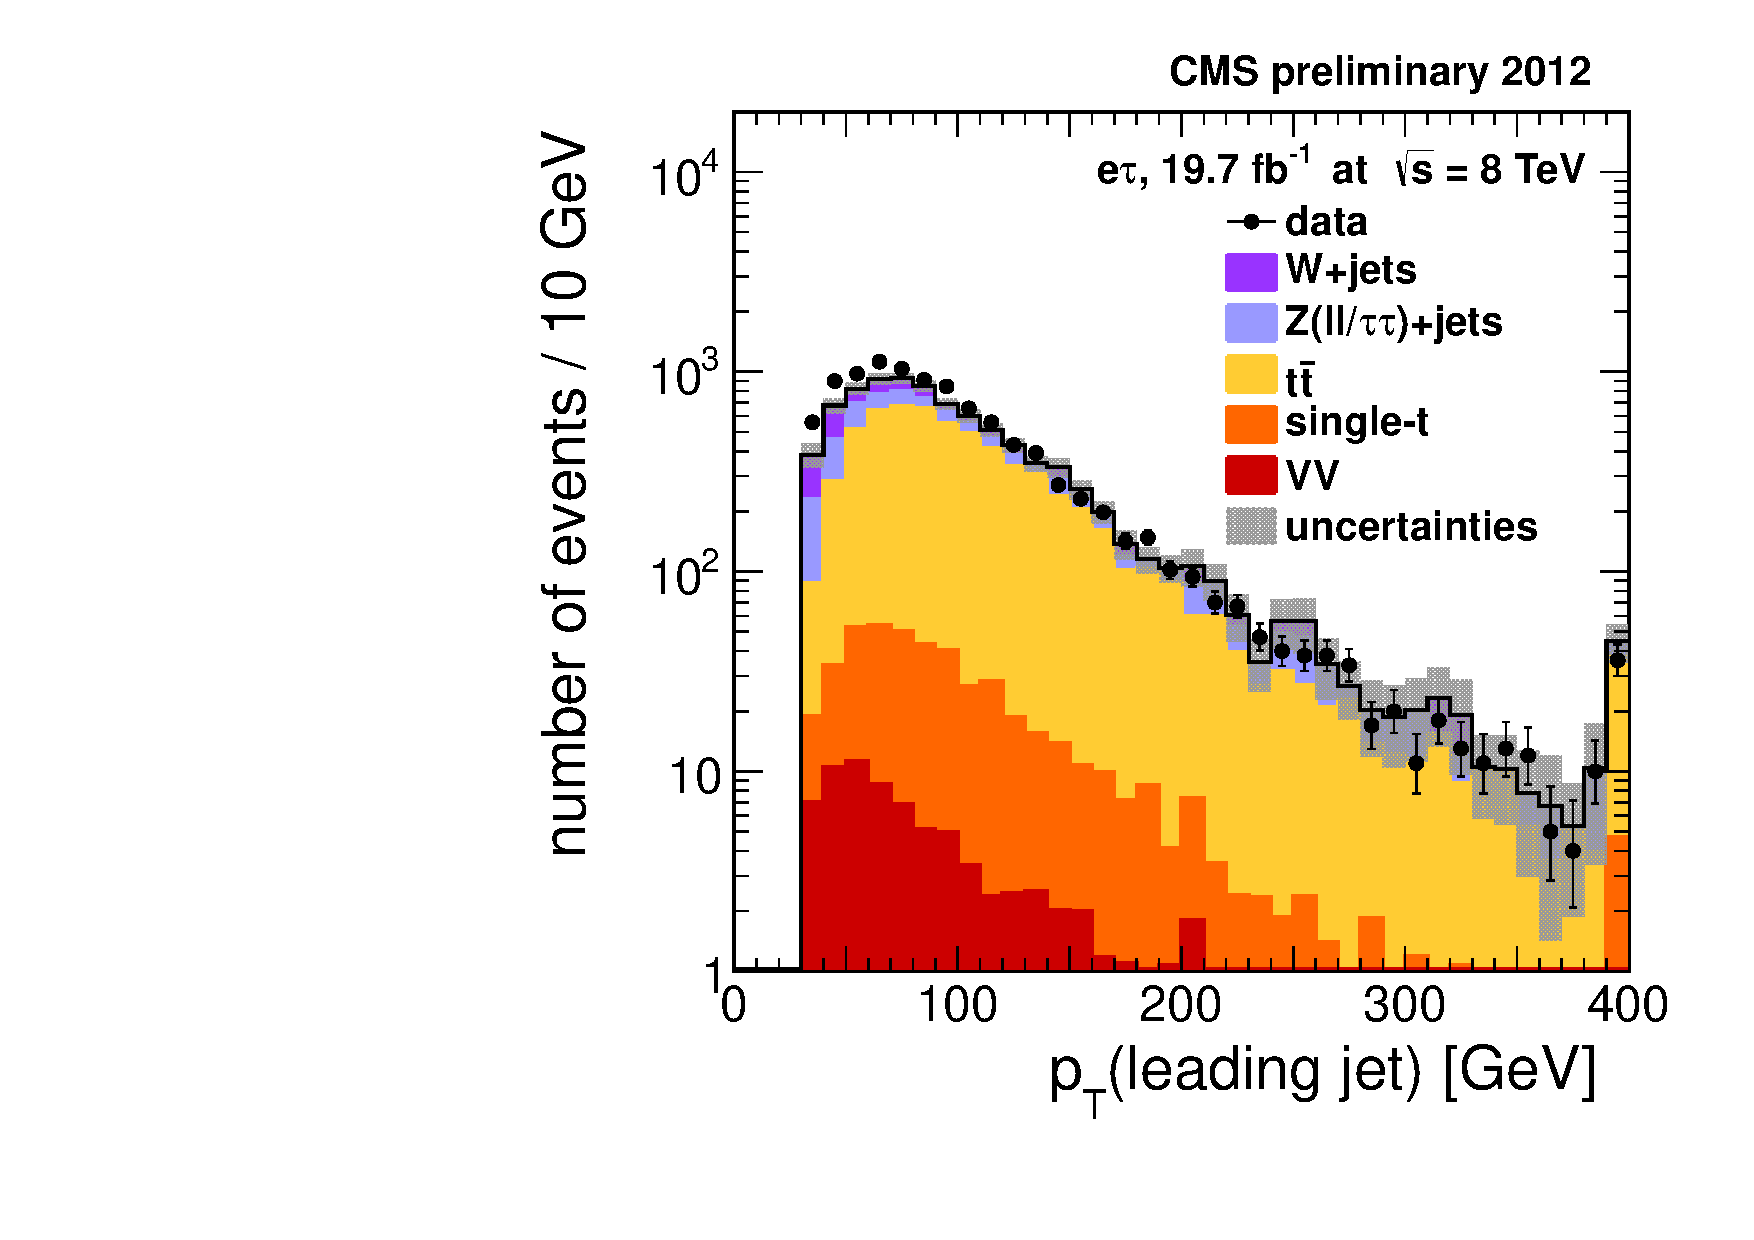
\includegraphics[width=0.49\textwidth]{figures/etau/jet1PtBTag.pdf}
    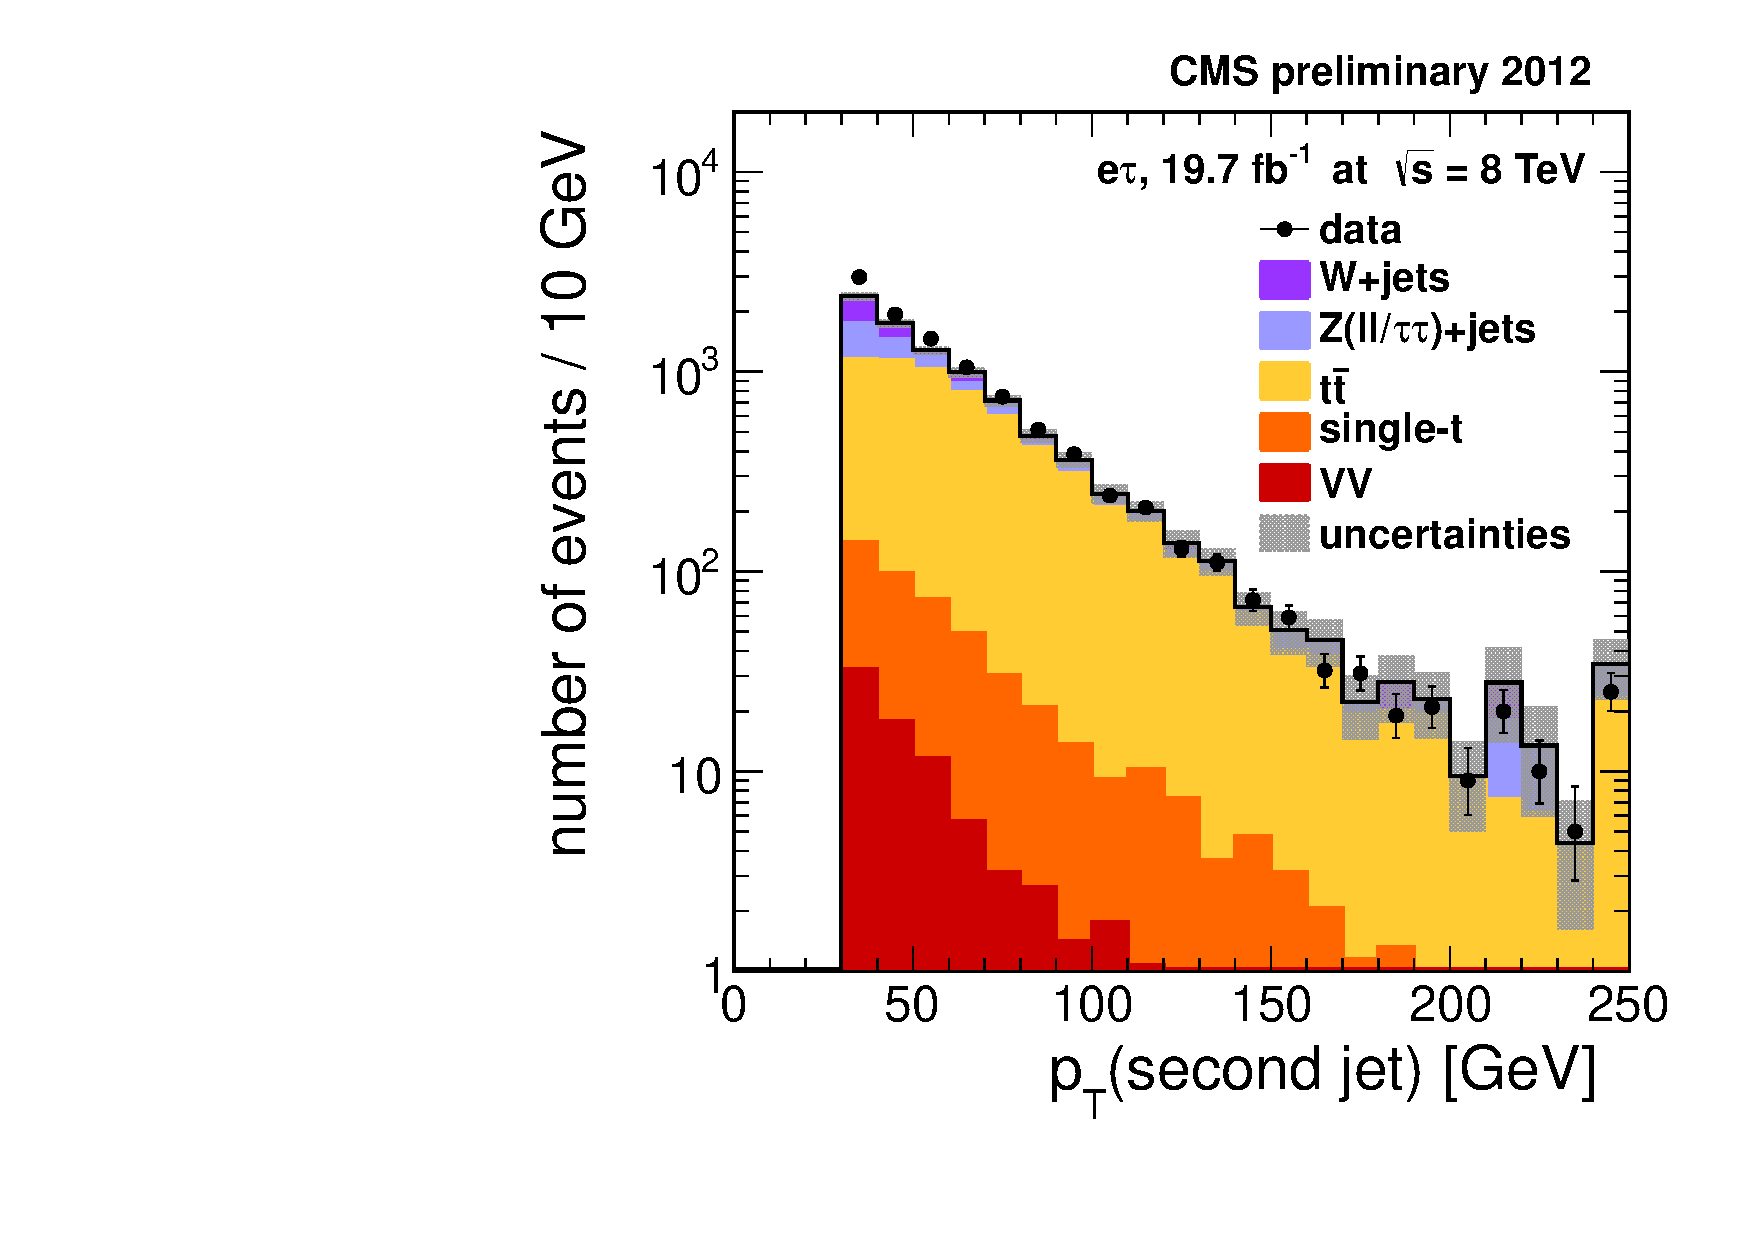
\includegraphics[width=0.49\textwidth]{figures/etau/jet2PtBTag.pdf} \\
    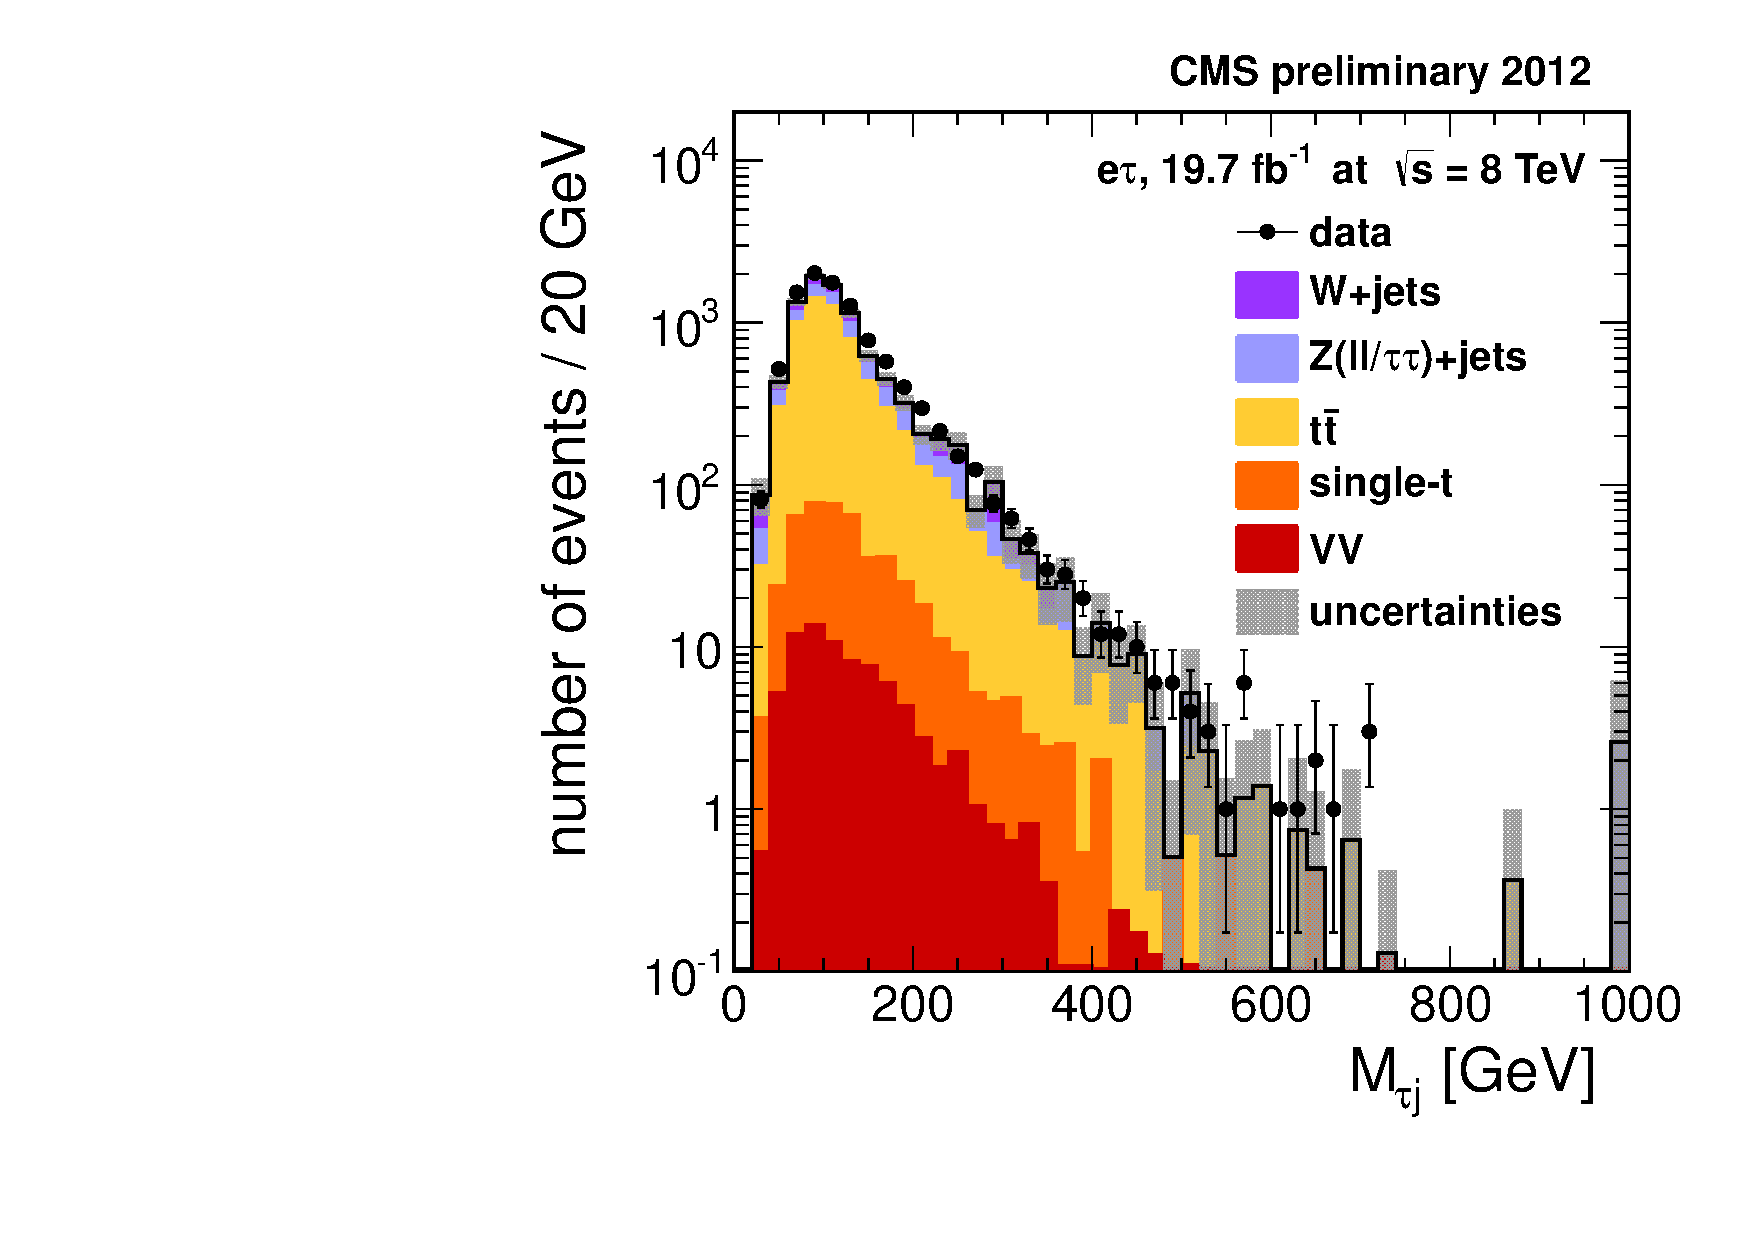
\includegraphics[width=0.49\textwidth]{figures/etau/finalMass.pdf}
    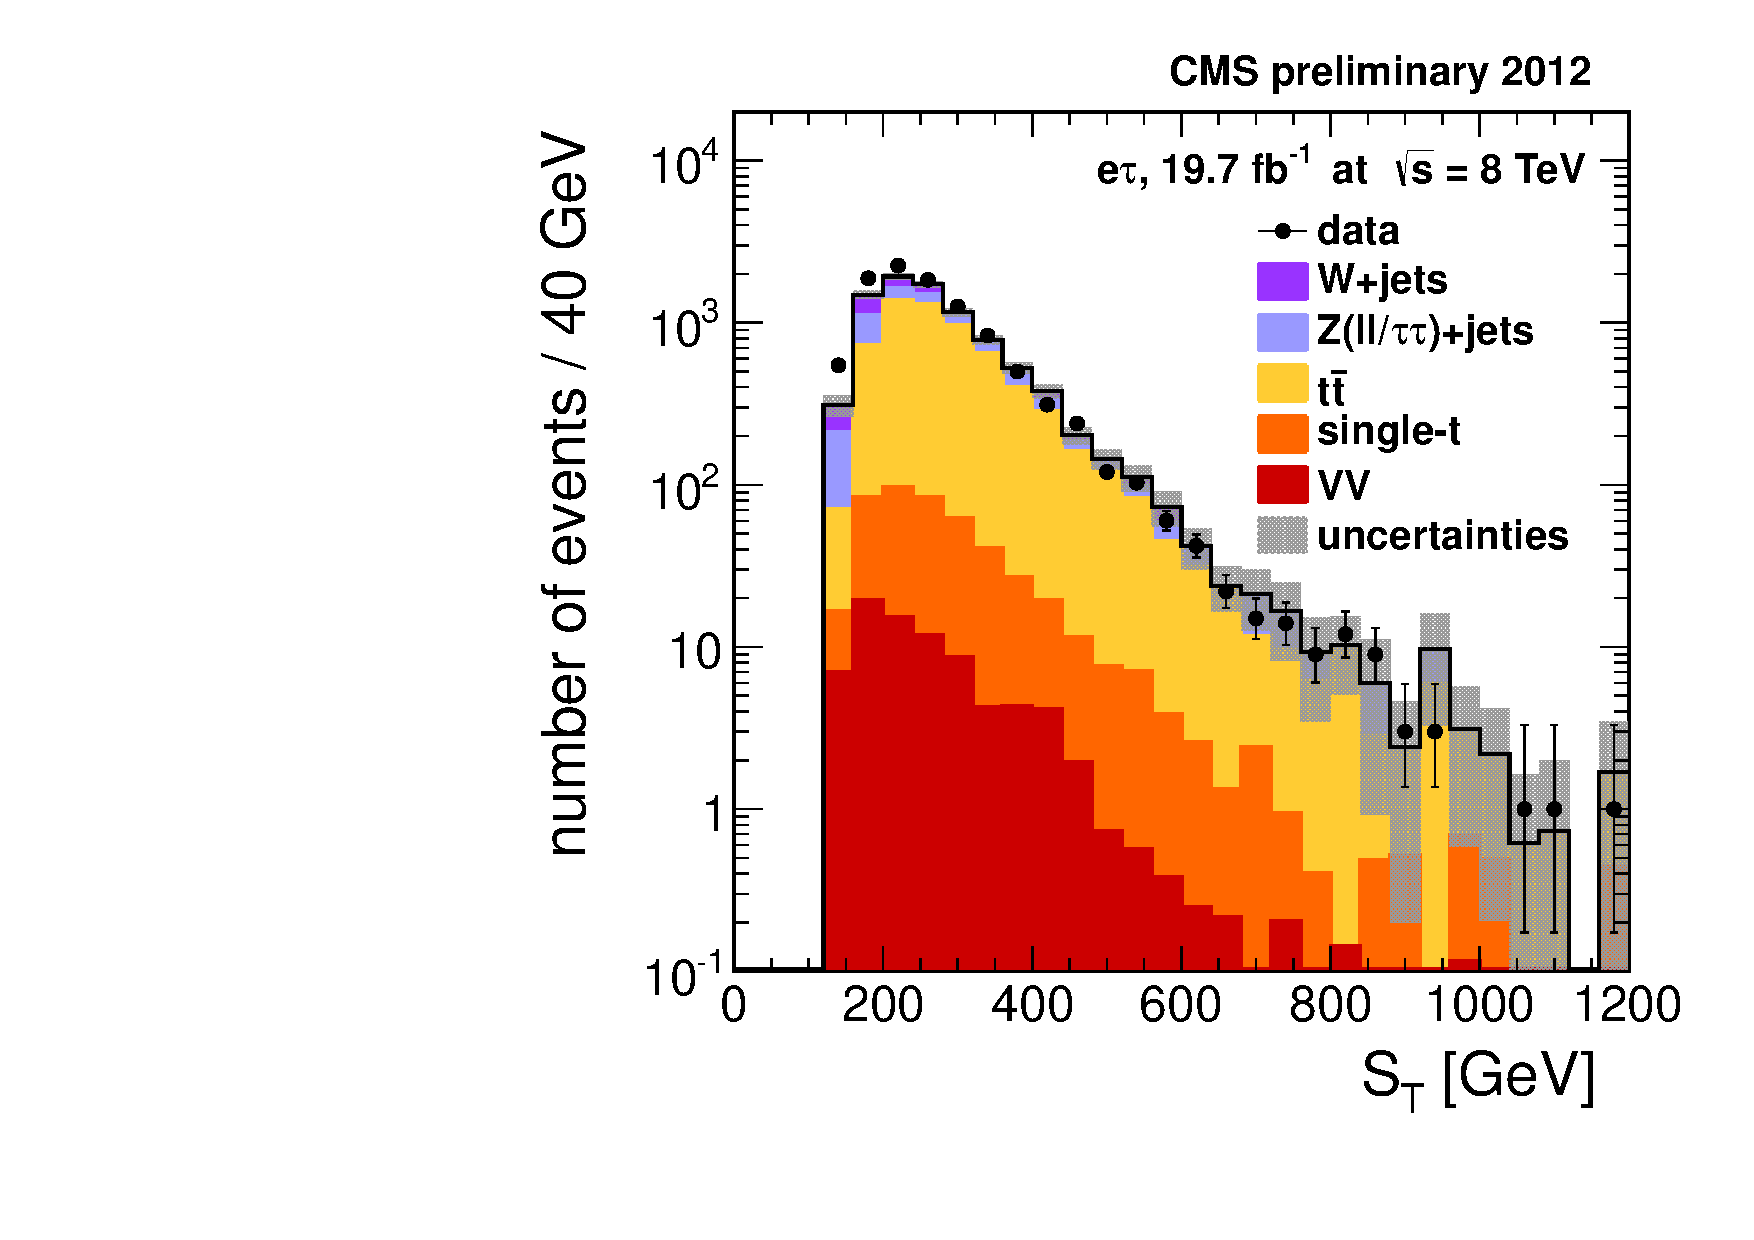
\includegraphics[width=0.49\textwidth]{figures/etau/STbjetBTag.pdf}
    \caption{Plots of various kinematic quantities comparing observed data and simulated backgrounds in the \etau channel after the main selection: the \pt spectra (top) of the first (left) and second (right) selected jets, \MassTJ (bottom left), and \ST (bottom right). The uncertainty band reflects the statistical uncertainty in the simulated backgrounds.}
    \label{fig:mainseletau}
  \end{center}
\end{figure}

\begin{figure}[hbtp]
  \begin{center}
    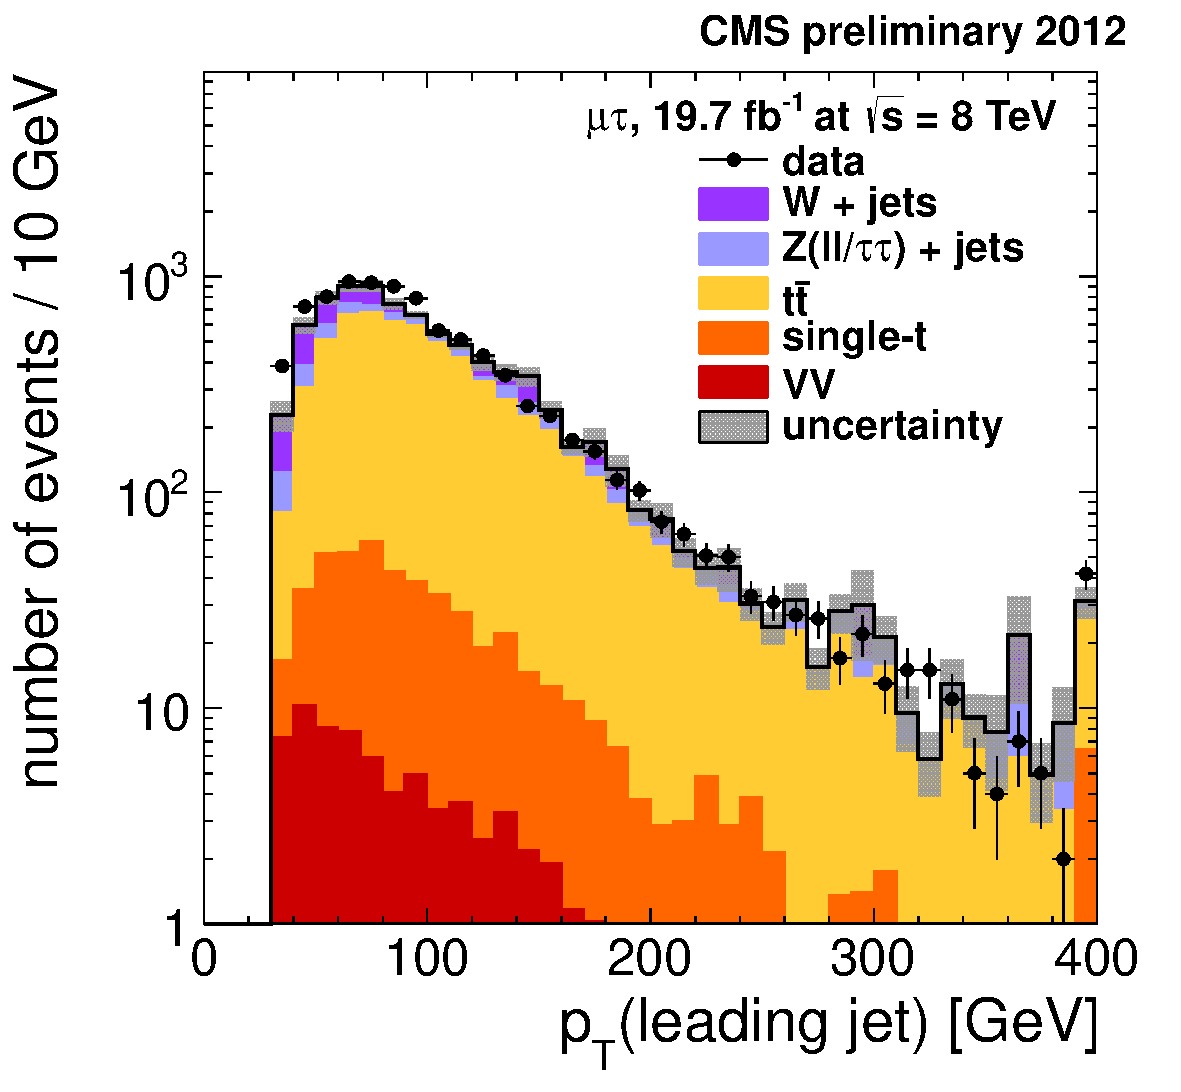
\includegraphics[width=0.49\textwidth]{figures/mutau/mainselection/leadseljetpt.pdf}
    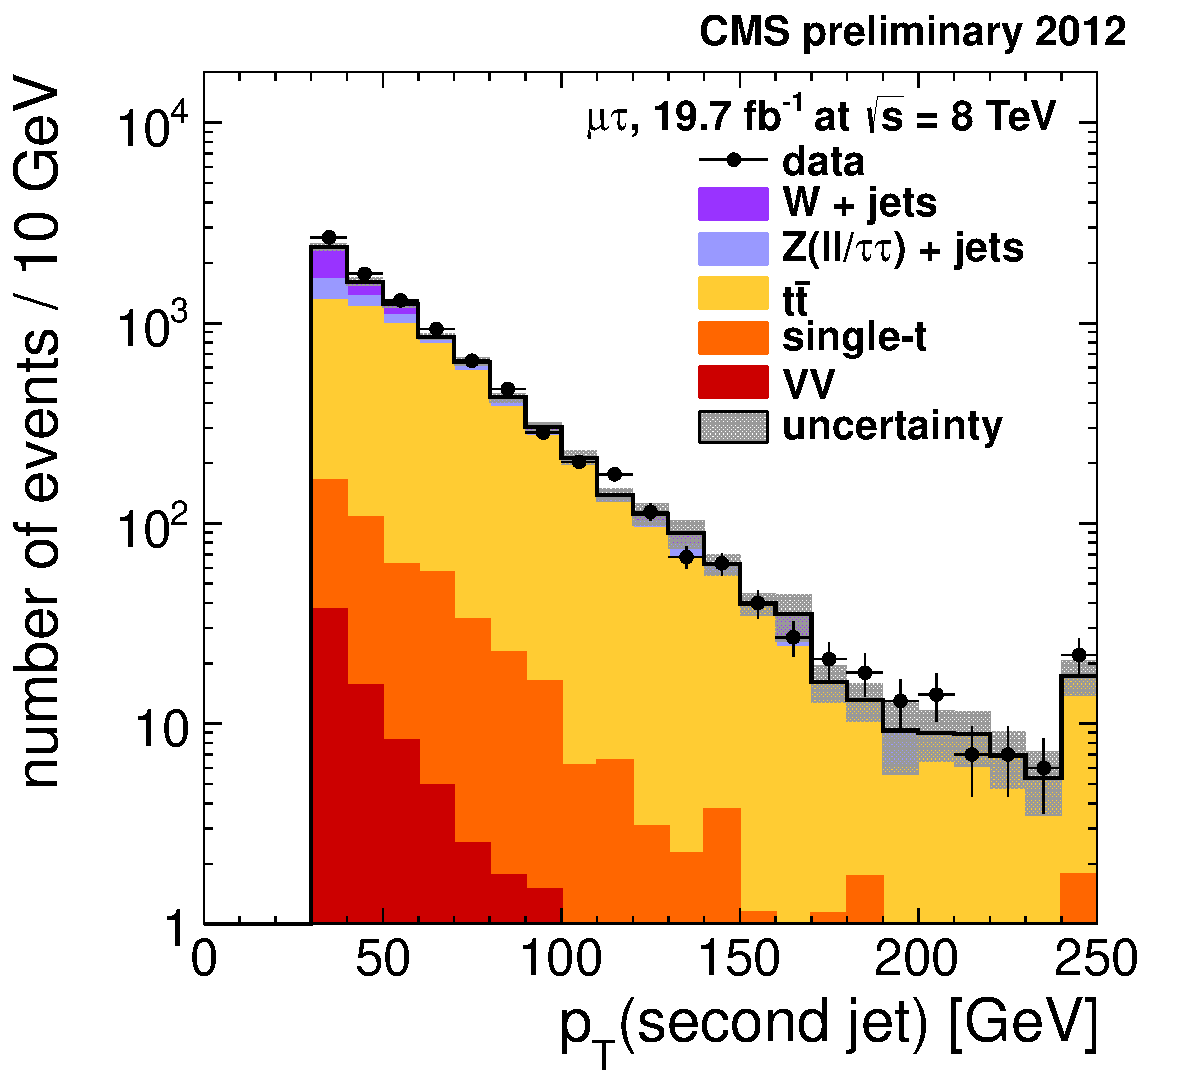
\includegraphics[width=0.49\textwidth]{figures/mutau/mainselection/secondseljetpt.pdf} \\
    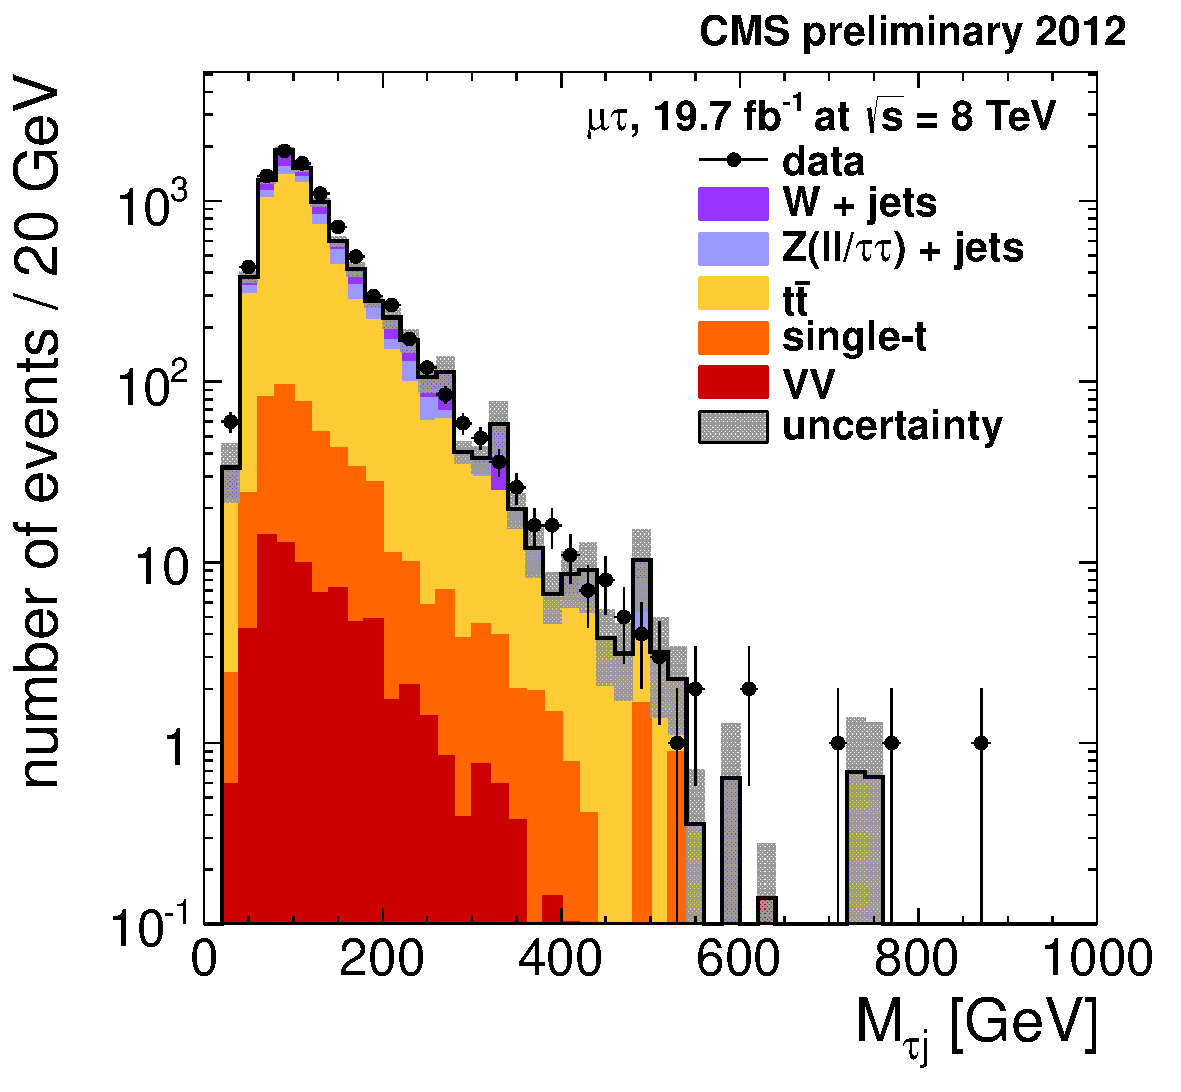
\includegraphics[width=0.49\textwidth]{figures/mutau/mainselection/masstaub.pdf}    
    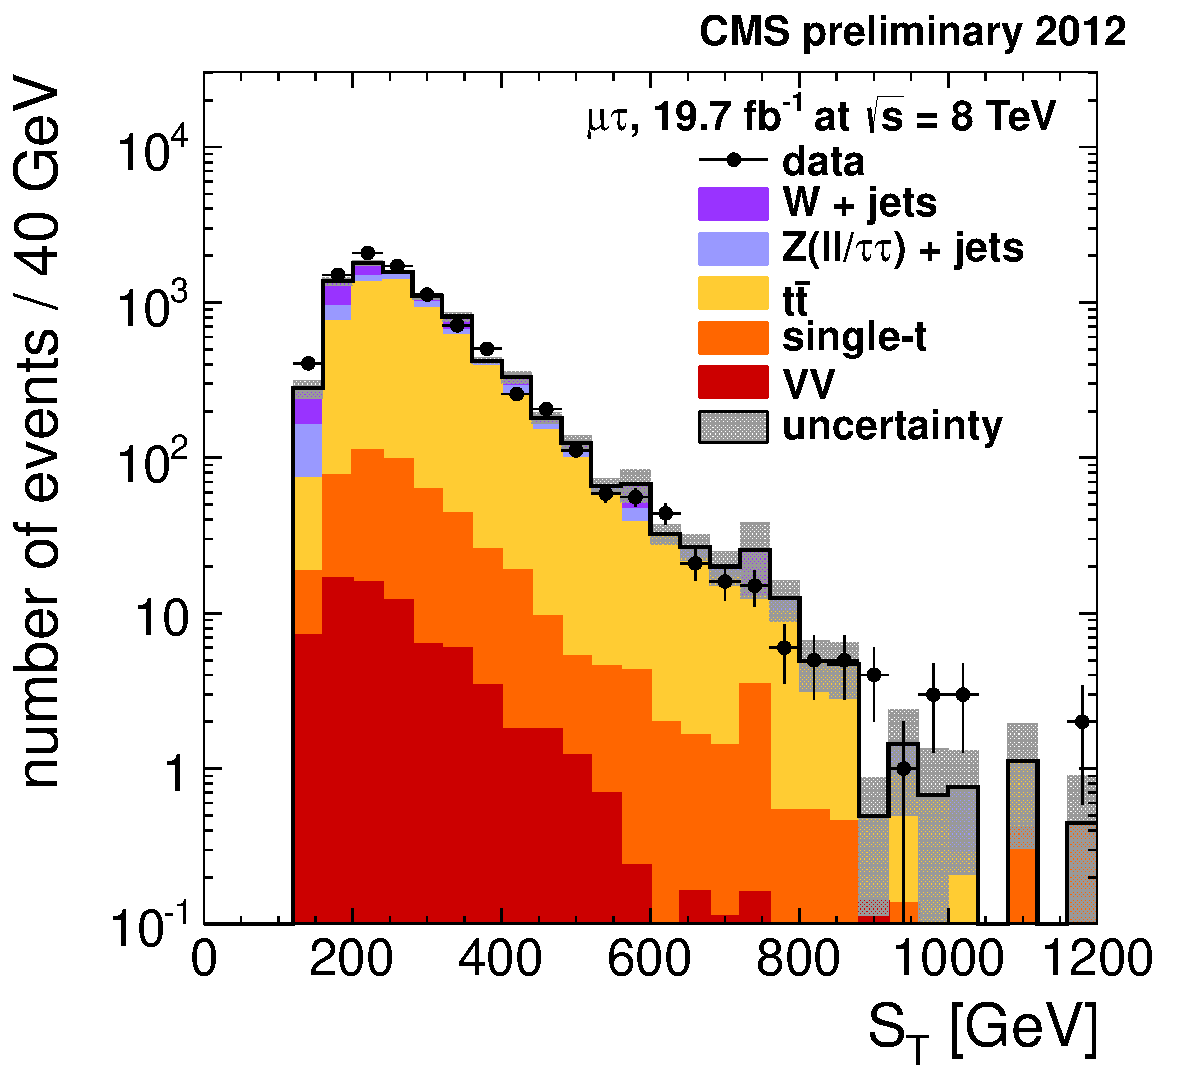
\includegraphics[width=0.49\textwidth]{figures/mutau/mainselection/st.pdf}
    \caption{Plots of various kinematic quantities comparing observed data and simulated backgrounds in the \mutau channel after the main selection: the \pt spectra (top) of the first (left) and second (right) selected jets, \MassTJ (bottom left), and \ST (bottom right). The uncertainty band reflects the statistical uncertainty in the simulated backgrounds.}
    \label{fig:mainselmutau}
  \end{center}
\end{figure}

\begin{table}[hbt]
  \begin{center}
    \begin{tabular}{|l|r@{$\,\pm\,$}r|r@{$\,\pm\,$}r|}
      \hline
      & \multicolumn{2}{c|}{\etau channel} & \multicolumn{2}{c|}{\mutau channel} \\
      \hline
      \W + jets                       & 1201.9 & 104.0   & 1285.8 & 122.7 \\
      \Z + jets                       & 1534.0 & 49.5    & 774.4 & 46.8   \\
      \ttbar                          & 5783.6 & 63.5    & 5699.5 & 64.4  \\
      Single \cPqt                    & 390.2  & 13.5    & 418.6 & 14.2   \\
      VV                              & 82.9   & 2.7     & 74.1 & 2.7     \\
      QCD multijets                   & (1226.0 & 131.0)\neghphantom{)}  & \multicolumn{2}{c|}{---}  \\
      \hline                                                 
      Total Bkg. (no QCD)             & 8992.6 & 141.2   & 8252.3 & 147.0 \\
      \hline
      \hline
      Data                            & \multicolumn{1}{r@{\hphantom{$\,\pm\,$}}}{10113\hphantom{.0}} & & \multicolumn{1}{r@{\hphantom{$\,\pm\,$}}}{8866\hphantom{.0}} &  \\
      \hline
    \end{tabular}
    \caption{The simulated background and observed event yields after the main selection in the \etau and \mutau channels. The statistical uncertainties are given for each simulated background. The contribution from the QCD multijets process is not taken into account in the total background yield. }
    \label{tab:eventyieldmainsel}
  \end{center}
\end{table}

%\clearpage

\subsection{Final Selections}

In the final stage of the selection for the leptoquark search, two additional requirements are applied. The selected hadronic tau must have $\pt>50\GeV$, and the selected events must have $\MassTJ>250\GeV$. This cut on the \MassTJ value is optimal for the expected limit based on the simulation for the entire range of leptoquark masses under consideration. The change in the kinematic properties of the signal for different mass values is taken into account when the \ST distribution is used to set $\text{CL}_{s}$ limits. The procedure for setting limits with a distribution is described in App. \ref{ch:limits}.

Slightly different final selection criteria are applied for the top squark search. Again, the selected hadronic tau must have $\pt>50\GeV$. Instead of a cut on \MassTJ, which is not a meaningful variable for the top squark $\lambda^{\prime}_{3jk}$ decay chain, the selected events are required to have $N_{\text{jets}}\geq5$. The expected final state of the top squark signal has $N_{\text{jet}}=6$, and though it was found that requiring $N_{\text{jets}}\geq6$ would maximize the expected limit based on the simulation, the number of both signal and background events passing that cut was greatly reduced. Because this would also reduce the number of events in the control regions used to estimate the major backgrounds, the corresponding increase in systematic uncertainty would render the limit indistinguishable from the $N_{\text{jets}}\geq5$ case. Thus, the slightly looser $N_{\text{jets}}$ cut was chosen. Given this cut, the \ST variable for the top squark search is defined as:
\begin{equation}
\label{eq:STstop}
\ST(\sTop) = \pt(\ell) + \pt(\tauh) + \pt(\text{b-jet}) + \sum_{i=1}^{4}\pt(\text{jet }i).
\end{equation}

Figure \ref{fig:finalcutscombined} shows the final selection variables for each search with both channels combined. Simulated signal distributions are added on top of the background to demonstrate the effect of the final selection cuts in removing background while preserving signal events. The common requirement $\pt(\tauh)>50\GeV$ is applied in these plots, and the major background yields are estimated from observed data. The background estimation techniques will be described in Sec. \ref{sec:background}.

\begin{figure}[hbt]
  \begin{center}
    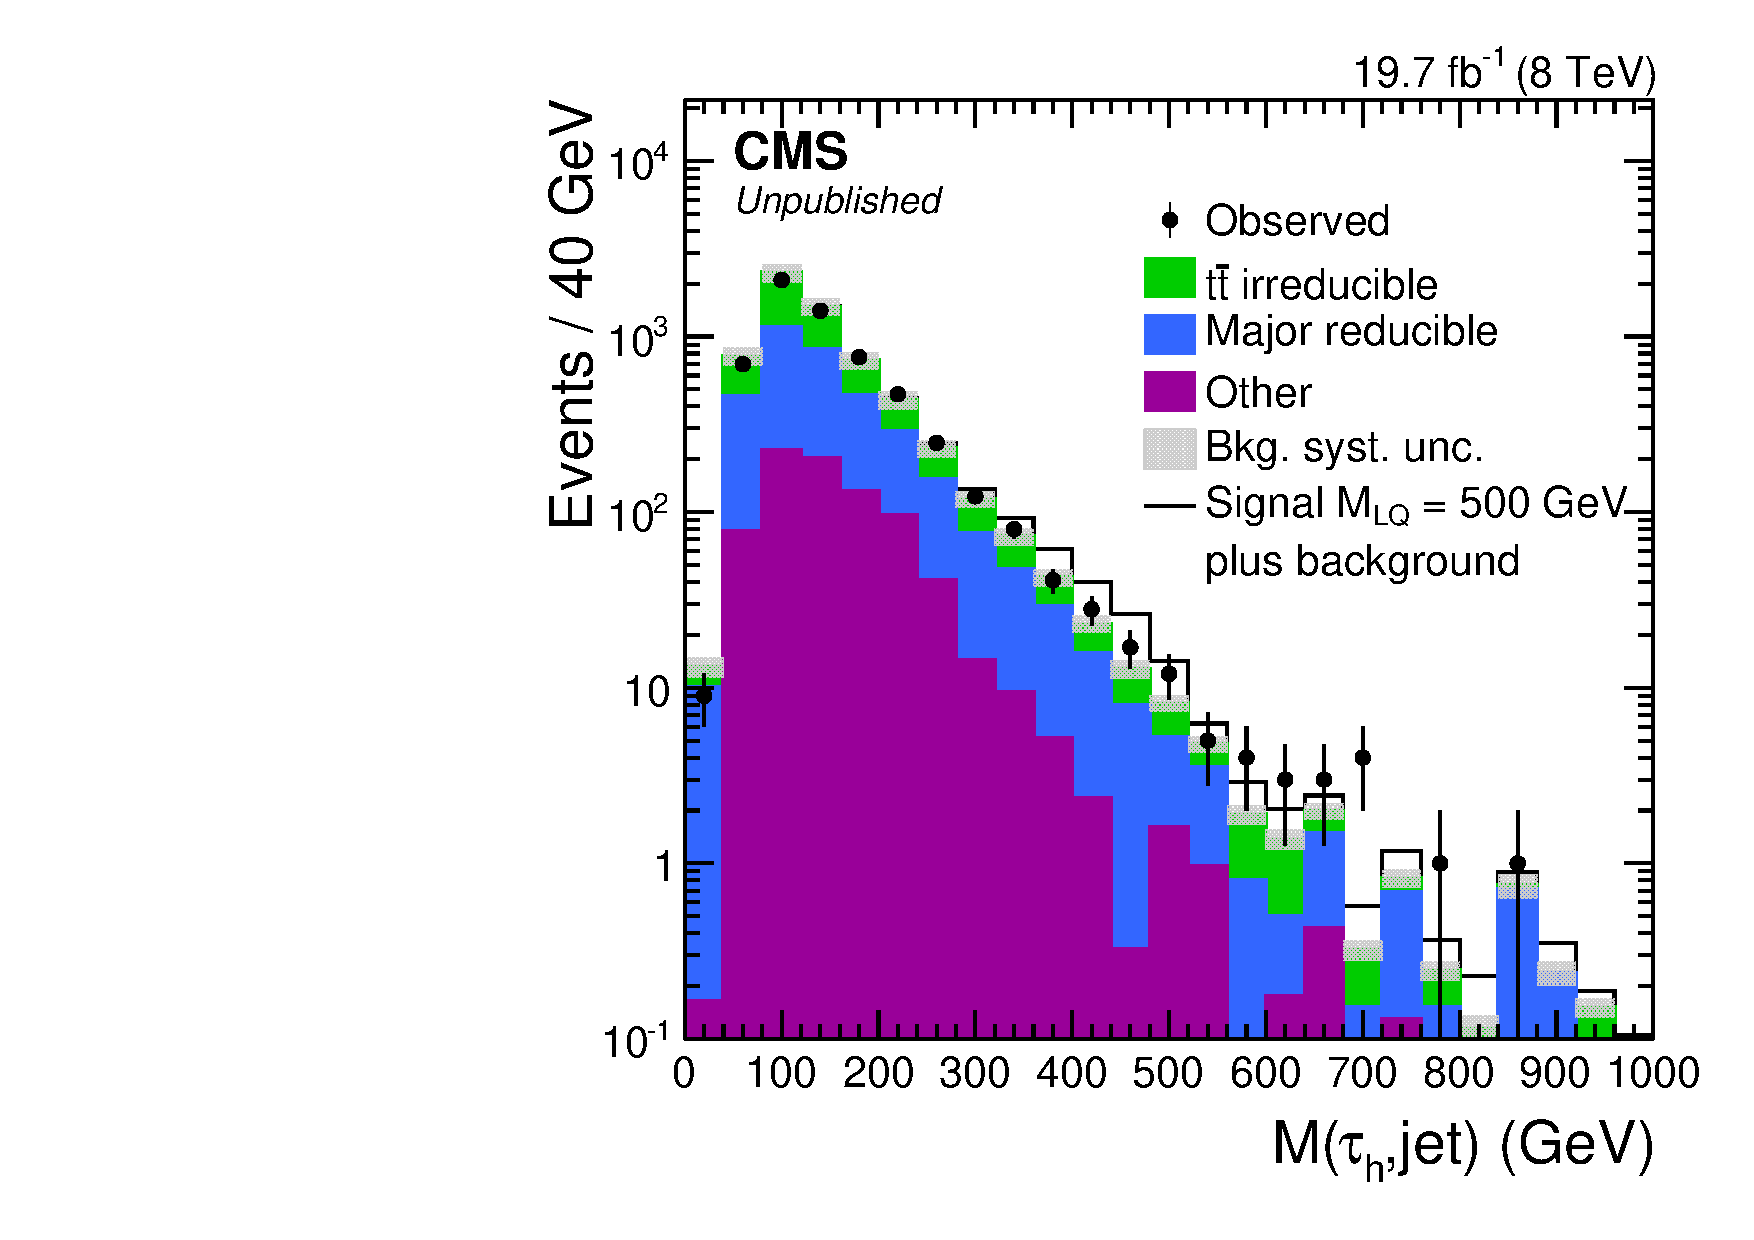
\includegraphics[width=0.49\textwidth]{figures/final/mtj_lq_log.pdf}
    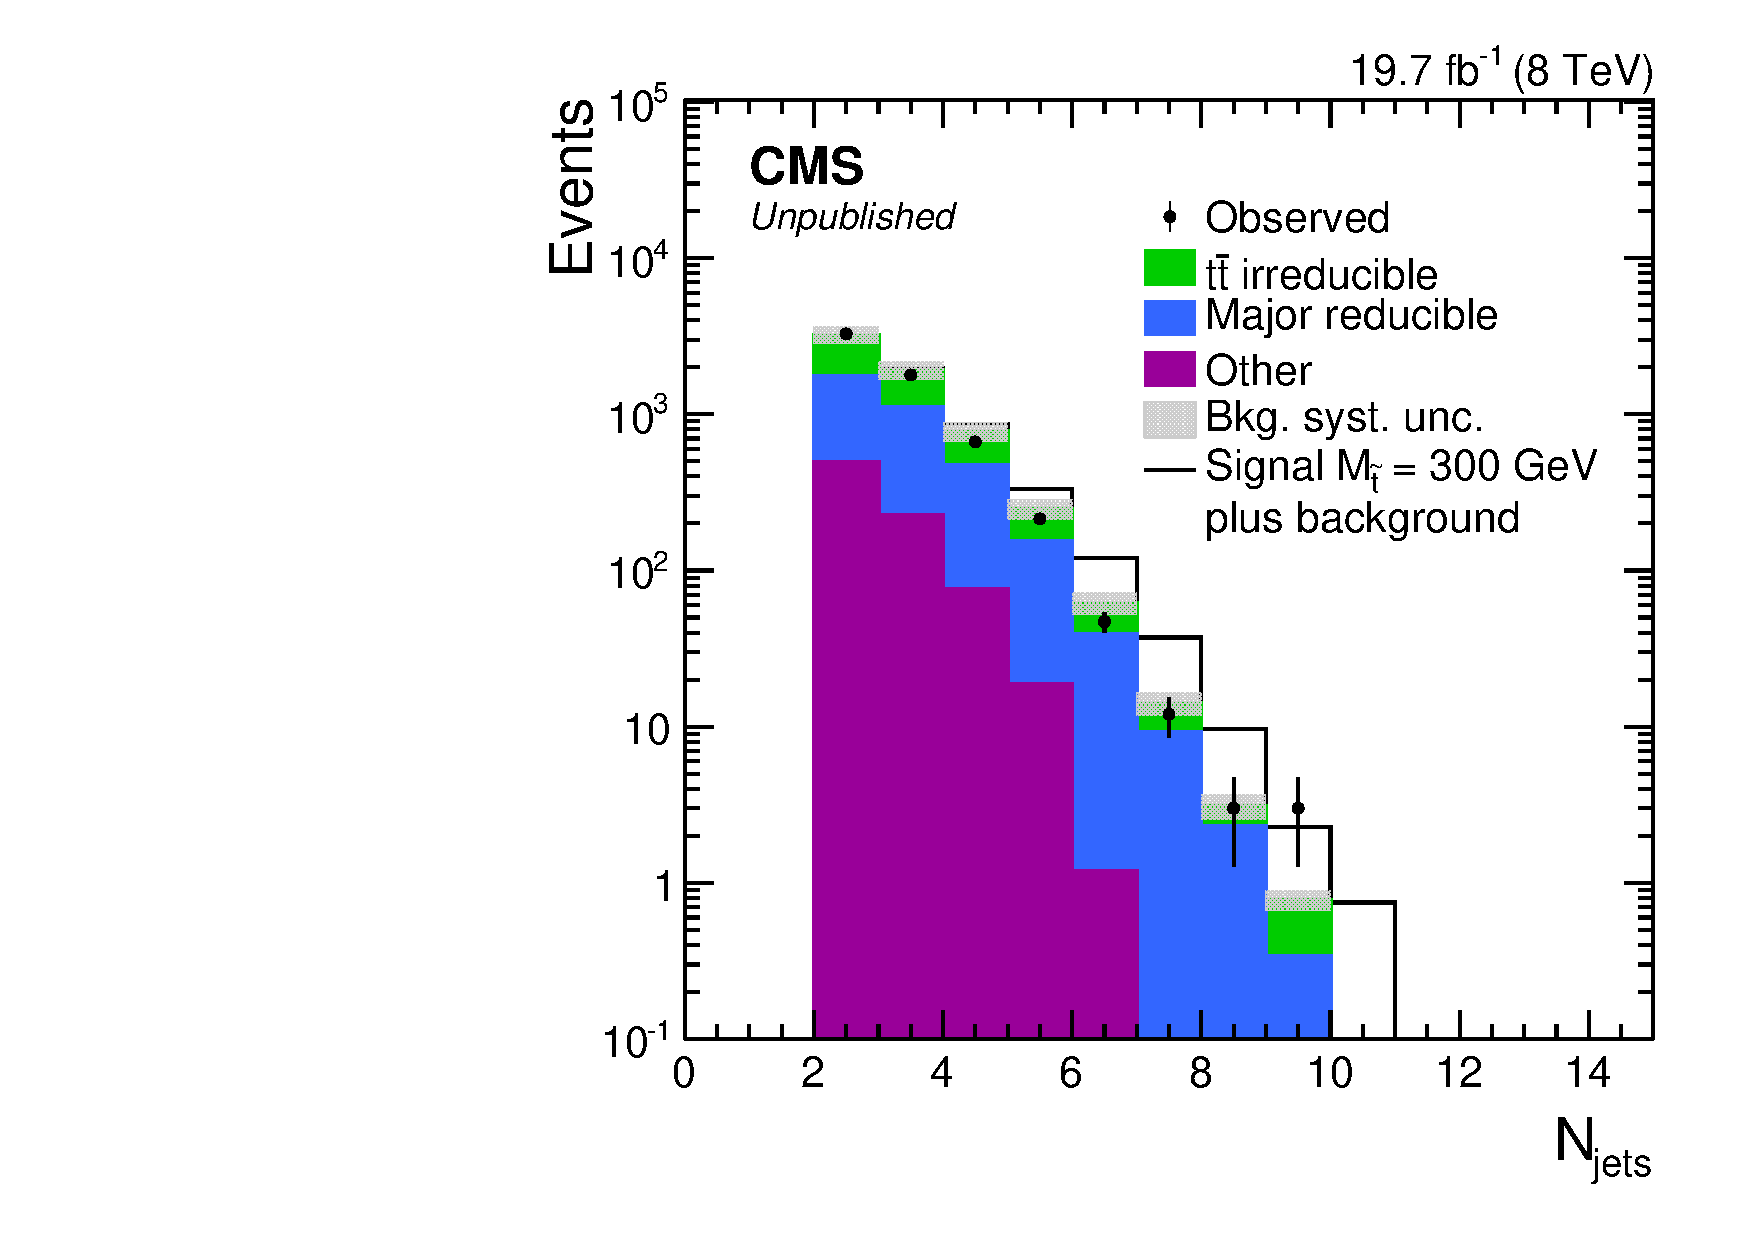
\includegraphics[width=0.49\textwidth]{figures/final/njets_lqd321_log.pdf}
    \caption{\MassTJ (left) and $N_{\text{jets}}$ (right) before the respective final selection cuts on these variables, with the \etau and \mutau channels combined. A signal sample for leptoquarks with a mass of 500\GeV (left) or top squarks with a mass of 300\GeV (right) is added on top of the background prediction. Both plots include the cut $\pt(\tauh)>50\GeV$ and the major backgrounds are estimated from observed data.}
    \label{fig:finalcutscombined}
  \end{center}
\end{figure}